% T12 C/D, chapitre 10 : Fonctions exponentielle et logarithme. Source : le livre « Terminales scientifiques » (ExpoLog/Lesona, ExpoLog/Exo).
% Les exercices tirés d’autres ouvrages ne sont pas repris (décision du 2 novembre 2026).

\TCDLessonStyleOn
\chapter{Fonction exponentielle et logarithme}
\section{Fonction exponentielle}
      \begin{defi}
      \index{Fonction!exponentielle}
            La \emph{fonction exponentielle} est l'unique fonction $f$ d\'efinie et d\'erivable sur $\mathbb{R}$ et v\'erifiant : 
                  \[   f' = f \qquad \text{ et } \qquad f(0) = 1   \,. \]
            On note la fonction par $\mathrm{exp}$.
      \end{defi}
      %
      \begin{prop}
            La fonction exponentielle peut en fait \^etre consid\'er\'ee comme une fonction puissance.
            Il existe un nombre r\'eel $e$ ($\simeq 2,718\,281\,828\,459\,045$) 
            tel que $\exp{x} = e^{x}$ pour tout $x\in\mathbb{Q}$.
            
            Ainsi, dor\'enavant, on consid\`erera la fonction exponentielle comme 
            une g\'en\'eralisation d'une fonction puissance.
            On d\'enotera alors $\exp{x}$ par $\expo{x}$.
      \end{prop}
      %
      \begin{thm}
            Soient $a$ et $b$ deux nombres r\'eels.
            \begin{itemize}
                  \item $\expo{0} = 1$
                  \item $\expo{a+b} = \expo{a} \cdot \expo{b}$
                  \item $\expo{-a} = \frac{1}{\expo{a}}$
                  \item $\expo{a-b} = \frac{\expo{a}}{\expo{b}}$
                  \item $\forall n \in \mathbb{Q},\ \left(\expo{a}\right)^n = \expo{na}$.
            \end{itemize}
      \end{thm}
      %
      \begin{prop}
            La fonction $\exp$ est d\'efinie sur $\mathbb{R}$.
            De plus, $\expo{x} > 0$ pour tout $x\in\mathbb{R}$ (car $\expo{x} = \left(\expo{x/2}\right)^2$ et $\expo{x/2}\,\expo{-x/2} = 1$, donc $\expo{x/2} \neq 0$).
            Comme $\exp' x = \exp x > 0$, alors la fonction $\exp$ est strictement croissante sur $\mathbb{R}$.
            Il suit que, pour tout $(x,y)\in\mathbb{R}^2$ :
                  \[
                        x<y \Rightarrow \expo{x} < \expo{y}      \;.
                  \]
      \end{prop}
      %
      \begin{thm}[Limites usuelles sur la fonction $\exp$]
            \begin{align*}
                  \lim_{x\rightarrow-\infty} \expo{x} & = 0     & \lim_{x\rightarrow+\infty} \expo{x} & = +\infty \\
                  \lim_{x\rightarrow-\infty} x \expo{x} & = 0   & \lim_{x\rightarrow+\infty} \frac{\expo{x}}{x} & = +\infty \\
                \intertext{ou plus g\'en\'eralement, pour tout $n\in\mathbb{N}$ (<< croissances compar\'ees >> : en $+\infty$, l'exponentielle l'emporte sur toute puissance de $x$)}
                  \lim_{x\rightarrow-\infty} x^n \expo{x} & = 0 & \lim_{x\rightarrow+\infty} \frac{\expo{x}}{x^n} & = +\infty\;.
            \end{align*}
            On a aussi 
                  \[
                        \lim_{x\rightarrow 0} \frac{\expo{x}-1}{x} = 1      \;.
                  \]
      \end{thm}
      %
      \paragraph{Fonctions compos\'ees avec la fonction exponentielle}
            Il suit de la formule de d\'erivation d'une fonction compos\'ee que 
            $\left( \expo{u} \right)' = u' \expo{u}$.
            Ainsi, $u$ et $\expo{u}$ ont m\^eme sens de variations.
            Par exemple, pour un r\'eel $k$, $\left(\expo{kx}\right)' = k\,\expo{kx}$.
      \paragraph{\'Etude de la fonction $\exp$}~\\
      Posons $f(x) = \expo{x}$.
            \begin{description}
            \item[Domaine de d\'efinition :] La fonction $\exp$ est d\'efinie sur $\mathbb{R} = ]-\infty,+\infty[$.
            \item[Limites aux bornes :] $\lim_{x\rightarrow -\infty} \expo{x} = 0$ et 
                                        $\lim_{x\rightarrow +\infty} \expo{x} = +\infty$
            \item[D\'eriv\'ee :] Pour tout $x\in\mathbb{R}$, $f'(x) = \expo{x}$.
            \item[Tableau des variations :]~\\[-1\baselineskip]
                  \begin{table}[H]
                  \centering
                        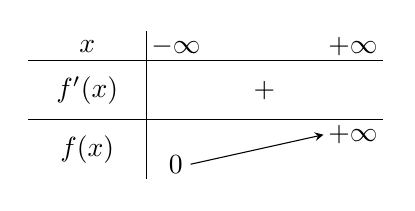
\begin{tikzpicture}[>=stealth,scale=.75]
                        \draw (-2,0) -- (4,0);
                        \draw (-2,-1) -- (4,-1);
                        \draw (0,.5) -- (0,-2);
                        \draw (-1,.25) node[] {$x$};
                        \draw (-1,-.5) node[] {$f'(x)$};
                        \draw (-1,-1.5) node[] {$f(x)$};
                        \draw (.5,.25) node[] {$-\infty$};
                        \draw (3.5,.25) node[] {$+\infty$};
                        \draw (2,-.5) node[] {$+$};
                        \draw (.5,-1.75) node[] {$0$};
                        \draw (3.5,-1.25) node[] {$+\infty$};
                        \draw[->] (.75,-1.75) -- (3,-1.25);
                        \end{tikzpicture}
                  \caption{Tableau des variations de la fonction exponentielle.}
                  \label{tab:variations expo}
                  \end{table}
            \item[Valeurs remarquables :] $f(0) = 1$ donc la courbe passe par le point de coordonn\'ees $(0,1)$.
                                          De plus, la d\'eriv\'ee en ce point est \'egale \`a $1$ :
                                          la tangente en ce point a pour \'equation $y = x + 1$,
                                          elle est parall\`ele \`a la premi\`ere bissectrice.
                                          $f(1) = \expo{}$ donc la courbe passe par le point de coordonn\'ees $(1,\expo{})$. 
            \item[Courbe repr\'esentative :]
                  Avant de tracer la courbe repr\'esentative de $f$, \'etudions d'abord ses branches infinies.
                  \begin{itemize}
                        \item Comme $\lim_{x\rightarrow-\infty} f(x) = 0$, 
                              alors la courbe admet la droite d'\'equation $y=0$ comme asymptote horizontale
                              au voisinage de $-\infty$.
                        \item Comme $\lim_{x\rightarrow+\infty} f(x) = +\infty$ et que
                              $\lim_{x\rightarrow+\infty} \frac{f(x)}{x} = +\infty$ alors
                              la courbe admet une branche parabolique de direction $(y'Oy)$ au voisinage de $+\infty$.
                  \end{itemize}
            \begin{figure}[h!]
            \centering
                  \begin{tikzpicture}[line cap=round,line join=round,>=stealth,scale=.9]
                  \draw[->,color=black] (-4.2,0) -- (5.24,0);
                  \foreach \x in {-4,-3,-2,-1,1,2,3,4,5}
                  \draw[shift={(\x,0)},color=black] (0pt,2pt) -- (0pt,-2pt) node[below] {\footnotesize $\x$};
                  \draw[->,color=black] (0,-4.2) -- (0,5.3);
                  \foreach \y in {-4,-3,-2,-1,1,2,3,4,5}
                  \draw[shift={(0,\y)},color=black] (2pt,0pt) -- (-2pt,0pt) node[left] {\footnotesize $\y$};
                  \draw[color=black] (0pt,-10pt) node[right] {\footnotesize $0$};
                  \clip(-4,-4) rectangle (5.7,5.7);
                  \draw[dashed] (0,2.718281828) -- (1,2.718281828);
                  \draw[dashed] (1,0) -- (1,2.718281828);
                  \draw[color=loko1, smooth,samples=100,domain=0:1.6, thick] 
                                                                  plot(\x,{2.718281828^(\x)}) node[fill=white] {$y=\expo x$};
                  \draw[color=loko1, smooth,samples=100,domain=0:5, thick] plot({-\x},{1/(2.718281828^(\x))});
                  \draw[color=loko3, smooth,samples=100,domain=-4:4, thick] plot(\x,{(\x)+1}) node[fill=white] {$y=x+1$};
                  \filldraw[fill=loko1, draw=loko2] (0,1) circle (.2em);
                  \filldraw[fill=loko1, draw=loko2] (1,2.718281828) circle (.2em);
                  \end{tikzpicture}
            \caption{Courbe repr\'esentative de la fonction $\exp$.}
            \label{fig:courbe exp}
            \end{figure}
            \end{description}
            

\section{Fonction Logarithme}
      \subsection{Logarithme n\'ep\'erien}
      \begin{defi}
      \index{Fonction!Logarithme neperien@Logarithme n\'ep\'erien}
            On a vu que la fonction exponentielle est continue (elle est m\^eme d\'erivable)
            et strictement croissante sur $\mathbb{R}$.
            Elle d\'efinit donc une bijection de $\mathbb{R}$ vers $\mathbb{R}^*_+$.
            On définit la fonction logarithme népérien comme étant la fonction r\'eciproque de la fonction exponentielle.
            Ainsi, 
            $\ln : \mathbb{R}^*_+   \rightarrow   \mathbb{R}$ v\'erifie :
                  \[
                        \left\lbrace
                              \begin{array}{ll}
                                    \forall x\in\mathbb{R}      ,&  \ln(\expo{x}) = x \\
                                    \forall x\in\mathbb{R}^*_+  ,&  \expo{\ln x} = x  \;.
                              \end{array}
                        \right.
                  \]
      \end{defi}
      Ainsi, dans un rep\`ere orthonorm\'e, la courbe de la fonction $\exp$ et celle de la fonction $\ln$ sont 
      sym\'etriques par rapport \`a la premi\`ere bissectrice (droite d'\'equation $y = x$).
            \begin{figure}[h!]
            \centering
                  \begin{tikzpicture}[line cap=round,line join=round,>=stealth,scale=.9]
                  \draw[->,color=black] (-4.2,0) -- (5.24,0);
                  \foreach \x in {-4,-3,-2,-1,1,2,3,4,5}
                  \draw[shift={(\x,0)},color=black] (0pt,2pt) -- (0pt,-2pt) node[below] {\footnotesize $\x$};
                  \draw[->,color=black] (0,-4.2) -- (0,5.3);
                  \foreach \y in {-4,-3,-2,-1,1,2,3,4,5}
                  \draw[shift={(0,\y)},color=black] (2pt,0pt) -- (-2pt,0pt) node[left] {\footnotesize $\y$};
                  \draw[color=black] (0pt,-10pt) node[right] {\footnotesize $0$};
                  \clip(-4,-4) rectangle (5.7,5.7);
                  \draw[color=loko2, smooth,samples=100,domain=0.001:5, thick] 
                        plot(\x,{ln((\x))}) node[fill=white,sloped,above left] {$y=\ln x$};
                  \draw[color=loko1, smooth,samples=100,domain=0:1.6, thick] 
                                                                  plot(\x,{2.718281828^(\x)}) node[fill=white] {$y=\expo x$};
                  \draw[color=loko1, smooth,samples=100,domain=0:5, thick] plot({-\x},{1/(2.718281828^(\x))});
                  \draw[color=loko3, smooth,samples=100,domain=-4:5, thick] plot(\x,{(\x)}) node[fill=white] {$y=x$};
                  \end{tikzpicture}
            \caption{Courbe des fonctions $\exp$ et $\ln$.}
            \label{fig:exp et ln}
            \end{figure}
      %
      \begin{rmk}[Valeurs remarquables]~\\[-1\baselineskip]
            \begin{itemize}
                  \item $\ln 1 = 0$ car $\expo{0} = 1$
                  \item $\ln \expo{} = 1$ car $\expo{1} = \expo{}$.
            \end{itemize}
            Comme la fonction exponentielle est une bijection continue et strictement croissante de $\mathbb{R}$ sur $]0,+\infty[$, 
            la fonction logarithme n\'ep\'erien est une bijection continue et strictement croissante de $]0,+\infty[$ sur $\mathbb{R}$.
            En particulier, $\ln x < 0$ pour $0 < x < 1$ et $\ln x > 0$ pour $x > 1$.
      \end{rmk}
      %
      \begin{prop}[Propri\'et\'es alg\'ebriques]
            Soient $a$, $b$ et $x$ des nombres r\'eels strictement positifs, $\lambda$ un r\'eel et $n$ un entier relatif.
            On a alors :\\
            \begin{align*}
                        \ln (a\cdot b) & = \ln a + \ln b                                                &       
                        \ln (a^n) & = n \cdot \ln a                                                     \\
                        \ln \frac{1}{a} & = - \ln a                                                     & 
                        \ln \frac{a}{b} & = \ln a - \ln b                                               \\
                        \ln a < \ln b & \iff a < b                                                      & 
                        \ln a = \ln b & \iff a = b                                                      \\
                        \ln x = \lambda & \iff x = \expo{\lambda}      & 
                        \ln x < \lambda & \iff x < \expo{\lambda}      
            \end{align*}
            et, pour tout r\'eel $t$ et tout r\'eel $\mu > 0$ :
            \begin{align*}
                        \expo{t} = \mu & \iff t = \ln{\mu} &
                        \expo{t} < \mu & \iff t < \ln{\mu} \;.
            \end{align*}
      \end{prop}
      %
      \begin{thm}[D\'eriv\'ee de la fonction $\ln$]
            La fonction logarithme n\'ep\'erien est d\'erivable sur $]0,+\infty[$ avec
                  \begin{equation*}
                        \left( \ln x \right)' = \frac{1}{x}      \;.
                  \end{equation*}
            \begin{proof}
                  Posons $f(x) = \expo{x}$. On sait alors que $f^{-1} (x) = \ln x$.
                  En utilisant la formule de d\'erivation de la fonction r\'eciproque, on a :
                        \begin{align*}
                              \left(f^{-1}\right)' (x)  & = \frac{1}{f' \left( f^{-1} (x) \right) }      \\
                              \left(\ln (x) \right)'    & = \frac{1}{\expo{\ln x}}                       \\
                              \left(\ln (x) \right)'    & = \frac{1}{x}                                  \,.
                        \end{align*}
            \end{proof}
      \end{thm}
      %
      \begin{thm}[Limites usuelles]~\\
                  \begin{align*}
                        \lim_{x\rightarrow 0^+} \ln x                & = -\infty            &
                        \lim_{x\rightarrow 0^+} x\cdot\ln x          & = 0                  \\
                        \lim_{x\rightarrow +\infty} \ln x            & = +\infty            &
                        \lim_{x\rightarrow +\infty} \frac{\ln x}{x}  & = 0                  
                  \end{align*}
                  Plus g\'en\'eralement (croissances compar\'ees), pour tout entier $n \geq 1$ :
                  $\displaystyle \lim_{x\rightarrow +\infty} \frac{\ln x}{x^n} = 0$ et $\displaystyle \lim_{x\rightarrow 0^+} x^n \ln x = 0$.
                  \[
                        \lim_{x\rightarrow 0} \frac{\ln (1 + x)}{x} = 1      \;.
                  \]
      \end{thm}
      %
      \paragraph{Fonctions compos\'ees avec la fonction logarithme n\'ep\'erien}
            Soit $u$ une fonction d\'erivable sur un intervalle $I$ tel que $u(x)>0$ pour tout $x\in I$.
            Il suit de la formule de d\'erivation d'une fonction compos\'ee que 
            $\left( \ln {u} \right)' = \frac{u'}{u}$.
            Ainsi, $u$ et $\ln{u}$ ont m\^eme sens de variations.
            Si $u$ est d\'erivable et ne s'annule pas sur $I$, on a de m\^eme
            $\left( \ln |u| \right)' = \frac{u'}{u}$ ; en particulier $\left(\ln|x|\right)' = \frac{1}{x}$ sur $]-\infty,0[$ et sur $]0,+\infty[$.
      %
            
      %
      \subsection{Logarithme de base quelconque}
            \begin{defi}[Logarithme d\'ecimal]
                  On d\'efinit la fonction logarithme d\'ecimal par :
                        \begin{equation*}
                              \begin{array}{rcl}
                                    \log :\ ]0,+\infty[ & \rightarrow & \mathbb{R}      \\
                                                     x & \mapsto     & \frac{\ln x}{\ln 10}
                              \end{array}
                        \end{equation*}
            \end{defi}
            %
            \begin{prop}
                  Si la fonction $\ln$ est la r\'eciproque de la fonction $x\mapsto \expo{x}$,
                  la fonction $\log$ peut \^etre consid\'er\'ee comme \'etant la r\'eciproque de la fonction $x\mapsto 10^x$.
                  
                  On a $\log 10 = 1$, $\log(10^p) = p$ pour tout entier $p$, et $\log$ v\'erifie les m\^emes propri\'et\'es alg\'ebriques que $\ln$ ;
                  sa d\'eriv\'ee est $x \mapsto \frac{1}{x \ln 10}$.
                  Si $n \geq 1$ est un nombre entier, l'\'ecriture d\'ecimale de $n$ comporte 
                  $\entiere{\log (n)}+1$ chiffres ($\mathrm{E}$ d\'esigne la partie enti\`ere) :
                  en effet, si $n$ a $p$ chiffres, $10^{p-1} \leq n < 10^p$, donc $p - 1 \leq \log n < p$.
                        \begin{ex}
                              Le nombre $2^{77\, 232\, 917} - 1$ est un nombre premier, d\'ecouvert en d\'ecembre 2017 par le projet de calcul GIMPS.
                              Comme $2^{77\, 232\, 917}$ n'est pas une puissance de $10$ (il n'est pas divisible par $5$),
                              $2^{77\, 232\, 917} - 1$ comporte le m\^eme nombre de chiffres que $2^{77\, 232\, 917}$.
                              Pour calculer le nombre de chiffres qu'il comporte, on effectue :
                                    \[
                                           \log (2^{77\, 232\, 917})
                                    =      \frac{\ln (2^{77\, 232\, 917})}{\ln 10} 
                                    =      \frac{77\, 232\, 917 \cdot \ln 2}{\ln 10}
                                    \simeq 23\,249\,424{,}67
                                    .
                                    \]
                              Ainsi, ce nombre comporte $23\,249\,425$ chiffres.
                        \end{ex}
            \end{prop}
            \begin{defi}[Logarithme de base $a$]
                  Soit $a$ un nombre r\'eel strictement positif et diff\'erent de $1$ (pour que $\ln a \neq 0$).
                  On d\'efinit la fonction logarithme de base $a$ par :
                        \begin{equation*}
                              \begin{array}{rcl}
                                    \log_a :\ ]0,+\infty[ & \rightarrow & \mathbb{R}                        \\
                                                        x & \mapsto     & \frac{\ln x}{\ln a}               \;.
                              \end{array}
                        \end{equation*}
            \end{defi}
            On a $\log_a 1 = 0$, $\log_a a = 1$, et $\log_{10} = \log$.
            La fonction $\log_a$ est croissante si $a > 1$, d\'ecroissante si $0 < a < 1$ ; c'est la r\'eciproque de la fonction $x \mapsto a^x$ d\'efinie ci-dessous.
      %
      \subsection{Fonction exponentielle de base $a$ et fonctions puissances}
            \begin{defi}[Exponentielle de base $a$]
            \index{Fonction!exponentielle de base a@exponentielle de base $a$}
                  Soit $a$ un r\'eel strictement positif. Pour tout r\'eel $x$, on pose
                  \[ a^x = \expo{x \ln a} \;. \]
                  Lorsque $x$ est un entier, on retrouve la puissance habituelle (car $\expo{n \ln a} = \left(\expo{\ln a}\right)^n = a^n$).
            \end{defi}
            \begin{prop}
                  Soient $a > 0$, $b > 0$ et $x$, $y$ des r\'eels. Alors
                  $a^{x+y} = a^x a^y$, $a^{-x} = \frac{1}{a^x}$, $\left(a^x\right)^y = a^{xy}$, $(ab)^x = a^x b^x$ et $\ln\left(a^x\right) = x \ln a$.

                  La fonction $x \mapsto a^x$ est d\'erivable sur $\mathbb{R}$ et $\left(a^x\right)' = (\ln a)\, a^x$.
                  \begin{itemize}
                        \item Si $a > 1$, elle est strictement croissante, $\lim_{x \rightarrow -\infty} a^x = 0$ et $\lim_{x \rightarrow +\infty} a^x = +\infty$ ;
                        \item si $0 < a < 1$, elle est strictement d\'ecroissante, $\lim_{x \rightarrow -\infty} a^x = +\infty$ et $\lim_{x \rightarrow +\infty} a^x = 0$ ;
                        \item si $a = 1$, elle est constante, \'egale \`a $1$.
                  \end{itemize}
                  Pour $a \neq 1$, $y = a^x \iff x = \log_a y$ (avec $y > 0$).
            \end{prop}
            \begin{prop}[Fonctions puissances]
                  Soit $\alpha$ un r\'eel. La fonction $x \mapsto x^\alpha = \expo{\alpha \ln x}$ est d\'efinie et d\'erivable sur $]0,+\infty[$ et
                  $\left(x^\alpha\right)' = \alpha\, x^{\alpha - 1}$.
                  Par exemple, $\sqrt{x} = x^{1/2}$ pour $x > 0$.
            \end{prop}
      %
      




\TCDLessonStyleOff
\clearpage
\providecommand{\ivec}{\vec{\imath}}
\providecommand{\jvec}{\vec{\jmath}}
\providecommand{\Oij}{$(O,\ivec,\jvec)$ }
%%%%%%%%%%%%%%%%%%%%%%%%%%%%%%%%%%%%%%%%%%%%%%%%%%%%%%%%%%%%%%%%%%%%%%%%%%%%%%%%%%%
%%%%%%%%%%%%%%%%%%%%%%%%%%%%%%%%%%%%%%%%%%%%%%%%%%%%%%%%%%%%%%%%%%%%%%%%%%%%%%%%%%%
\section{Exercices}
%%%%%%%%%%%%%%%%%%%%%%%%%%%%%%%%%%%%%%%%%%%%%%%%%%%%%%%%%%%%%%%%%%%%%%%%%%%%%%%%%%%
\begin{exo}
\label{exo:el quotient expo}
\begin{description}
\item[Partie A.] On consid\`ere la fonction $\varphi$ d\'efinie sur $\mathbb{R}$ par $\varphi(x) = 1 - (x+2)\,\expo{x}$.
      \begin{enumerate}
      \item Calculer les limites de $\varphi$ en $-\infty$ et en $+\infty$.
      \item \'Etudier le sens de variation de $\varphi$ et dresser son tableau de variation.
      \item Montrer que l'\'equation $\varphi(x) = 0$ admet une unique solution $\alpha$ dans $\mathbb{R}$ et que
            $-0{,}45 < \alpha < -0{,}44$.
      \item En d\'eduire le signe de $\varphi(x)$ suivant les valeurs de $x$.
      \end{enumerate}
\item[Partie B.] Soit $f$ la fonction d\'efinie sur $\mathbb{R}$ par $f(x) = \frac{x+3}{\expo{x} + 1}$ et
      $(\mathcal{C})$ sa courbe repr\'esentative dans un rep\`ere orthonorm\'e $(O , \ivec , \jvec )$ d'unit\'e $2$~cm.
      \begin{enumerate}
      \item Calculer les limites de $f$ en $-\infty$ et en $+\infty$. Interpr\'eter graphiquement la limite en $+\infty$.
      \item Montrer que, pour tout r\'eel $x$, $f'(x) = \frac{\varphi(x)}{\left(\expo{x}+1\right)^2}$.
            Dresser le tableau de variation de $f$.
      \item Montrer que $f(\alpha) = \alpha + 2$ et en d\'eduire un encadrement de $f(\alpha)$.
      \item Montrer que la droite $(\mathcal{D})$ d'\'equation $y = x + 3$ est asymptote \`a $(\mathcal{C})$ en $-\infty$,
            puis \'etudier la position de $(\mathcal{C})$ par rapport \`a $(\mathcal{D})$.
      \item Pr\'eciser les points d'intersection de $(\mathcal{C})$ avec les axes de coordonn\'ees,
            puis tracer $(\mathcal{D})$ et $(\mathcal{C})$.
      \end{enumerate}
\end{description}
\end{exo}
%%%%%%%%%%%%%%%%%%%%%%%%%%%%%%%%%%%%%%%%%%%%%%%%%%%%%%%%%%%%%%%%%%%%%%%%%%%%%%%%%%%
\begin{exo} ~ \newline
\label{exo:el raccord ln exp}
Soit la fonction num\'erique $f$ d\'efinie sur l'intervalle $]-1 \; ; \; +\infty[$ par :
\begin{displaymath}
f(x) =
\left\lbrace
\begin{tabular}{lll}
$ - x + 2 \ln (x + 1) $ & si & $ x \in \; ] -1 \; ; \; 0[ $ \\
$ x - 1 + \expo{-x} $ & si & $ x \in [0 \; ; \; + \infty[ $.
\end{tabular}
\right.
\end{displaymath}
On note par $(\mathscr{C})$ sa courbe repr\'esentative dans un rep\`ere orthonorm\'e \Oij d'unit\'e 2 cm.
\begin{enumerate}
\item Montrer que $f$ est continue en $0$.
\item Montrer que $\lim_{x \rightarrow 0^-} \frac{f(x) - f(0)}{x - 0} = 1$ et
      $\lim_{x \rightarrow 0^+} \frac{f(x) - f(0)}{x - 0} = 0$.
      Que peut-on en conclure sur $f$\,?
\item \begin{enumerate}
      \item Calculer $\lim_{x \rightarrow -1^+} f(x)$ et $\lim_{x \rightarrow +\infty} f(x)$.
      \item \'Etudier le signe de $f'(x)$ sur les intervalles $]-1 \; ; \; 0[$ et $] 0 \; ; \; +\infty[$.
      \item Dresser le tableau des variations de $f$.
      \end{enumerate}
\item Montrer que la droite $(\mathcal{D})$ d'\'equation $y = x- 1$ est asymptote \`a $(\mathscr{C})$ au voisinage de $+\infty$.
\item Tracer $(\mathscr{C})$ et $(\mathcal{D})$ dans le m\^eme rep\`ere \Oij en pr\'ecisant les demi-tangentes \`a l'origine.
\item Soit $g$ la restriction de $f$ \`a l'intervalle $I = [ 0 \; ; \; +\infty[$.
      \begin{enumerate}
      \item Montrer que $g$ admet une r\'eciproque $g^{-1}$ dont on d\'eterminera l'ensemble de d\'efinition.
      \item Repr\'esenter $g^{-1}$ dans le m\^eme rep\`ere que $(\mathscr{C})$.
      \end{enumerate}
\end{enumerate}

\end{exo}
%%%%%%%%%%%%%%%%%%%%%%%%%%%%%%%%%%%%%%%%%%%%%%%%%%%%%%%%%%%%%%%%%%%%%%%%%%%%%%%%%%%
\begin{exo} ~ \newline
\label{exo:el point anguleux}
Soit $f$ la fonction d\'efinie sur $\mathbb{R}$ par
\begin{displaymath}
f(x) =
\left\lbrace
\begin{matrix}
x - 2 - \ln ( \expo{} - x) & \text{ si } & x < 0     \\
\expo{x} \; (x^2 - 3)   & \text{ si } & x \geq 0  \; .
\end{matrix}
\right.
\end{displaymath}
On note $(\mathscr{C})$ sa courbe repr\'esentative dans un rep\`ere orthonorm\'e \Oij d'unit\'e 1~cm.
\begin{enumerate}
\item \begin{enumerate}
      \item \'Etudier la continuit\'e de $f$ en $0$.
      \item Montrer que $f$ est d\'erivable \`a gauche en $0$ et que $f'_g (0) = 1 + \frac{1}{\expo{}}$.
      \item Montrer que $f$ est d\'erivable \`a droite en $0$ et calculer $f'_d (0)$. Que peut-on en conclure\,?
      \end{enumerate}
\item \begin{enumerate}
      \item \'Etudier les variations de $f$.
      \item D\'eterminer les branches infinies de $(\mathscr{C})$.
      \item Montrer que $(\mathscr{C})$ coupe la premi\`ere bissectrice en un unique point, dont l'abscisse $\alpha$ appartient \`a $\left] \sqrt{3} \; ; \; 2 \right[$.
            (On ne demande pas de calculer la valeur de $\alpha$.)
      \end{enumerate}
\item Tracer la courbe $(\mathscr{C})$ en pr\'ecisant les demi-tangentes au point d'abscisse $0$.
\end{enumerate}
\end{exo}
%%%%%%%%%%%%%%%%%%%%%%%%%%%%%%%%%%%%%%%%%%%%%%%%%%%%%%%%%%%%%%%%%%%%%%%%%%%%%%%%%%%
\begin{exo} ~ \newline
\label{exo:el x plus lnx sur x}
On consid\`ere la fonction $f$ d\'efinie sur $I = ]0 \; ; \; +\infty[$ par $f(x) = x + \frac{2 \; \ln (x) }{x}$.
On d\'esigne par $(\mathscr{C})$ sa courbe repr\'esentative dans un rep\`ere orthonorm\'e \Oij d'unit\'e 1~cm.
\begin{enumerate}
\item Soit $g$ la fonction d\'efinie sur $]0 \; ; \; +\infty[$ par $g(x) = x^2 + 2 - 2 \; \ln (x)$.
      \'Etudier les variations de $g$ et en d\'eduire le signe de $g(x)$.
\item \begin{enumerate}
      \item Calculer les limites de $f$ aux bornes de son domaine de d\'efinition.
      \item Dresser le tableau des variations de $f$.
      \item Montrer que la droite $(\mathcal{D})$ d'\'equation $y = x$ est asymptote \`a $(\mathscr{C})$ et
            \'etudier la position de $(\mathscr{C})$ par rapport \`a $(\mathcal{D})$.
      \item On d\'esigne par $A$ le point de $(\mathscr{C})$ o\`u la tangente $(T)$ est parall\`ele \`a $(\mathcal{D})$.
            D\'eterminer les coordonn\'ees du point $A$.
      \item Tracer $(\mathscr{C})$, $(\mathcal{D})$ et $(T)$ dans le rep\`ere \Oij.
      \end{enumerate}
\item Montrer que l'\'equation $f(x) = 0$ admet une solution unique $\alpha$ et
      montrer que $\alpha \in \left] \frac{1}{2} \; ; \; 1 \right[$.
\end{enumerate}
\end{exo}
%%%%%%%%%%%%%%%%%%%%%%%%%%%%%%%%%%%%%%%%%%%%%%%%%%%%%%%%%%%%%%%%%%%%%%%%%%%%%%%%%%%
\begin{exo}
\label{exo:el x ln}
\begin{description}
\item[A.] On consid\`ere la fonction $g$ d\'efinie sur $]0 \; ; \; +\infty[$ par
      $g(x) = \ln \left( \frac{x+1}{x} \right) - \frac{1}{x+1}$.
      \begin{enumerate}
      \item D\'eterminer les limites de $g$ aux bornes de son domaine de d\'efinition.
      \item Dresser le tableau de variation de $g$.
            En d\'eduire le signe de $g(x)$ pour $x > 0$.
      \end{enumerate}
\item[B.] On consid\`ere la fonction $f$ d\'efinie sur $]0 \; ; \; +\infty[$ par
      $f(x) = x \; \ln \left( \frac{x+1}{x} \right)$.
      \begin{enumerate}
      \item Calculer les limites de $f$ aux bornes de son domaine de d\'efinition.
      \item Dresser le tableau de variation de la fonction $f$.
      \item Tracer la courbe $(\mathscr{C})$ repr\'esentative de $f$.
      \end{enumerate}
\end{description}
\end{exo}
%%%%%%%%%%%%%%%%%%%%%%%%%%%%%%%%%%%%%%%%%%%%%%%%%%%%%%%%%%%%%%%%%%%%%%%%%%%%%%%%%%%
\begin{exo} ~ \newline
\label{exo:el ln valeur absolue}
Soit $f$ la fonction d\'efinie par $f(x) = - \frac{x}{2} + \ln \left| \frac{x-1}{x} \right| $.
\begin{enumerate}
\item D\'eterminer l'ensemble de d\'efinition $\mathcal{D}_f$ de $f$.
\item \'Etudier les variations de $f$.
\item On d\'esigne par $(\mathscr{C})$ la courbe repr\'esentative de $f$ dans un rep\`ere orthonorm\'e \Oij d'unit\'e 2~cm.
      Montrer que la droite $(\mathcal{D})$ d'\'equation $y = -\frac{x}{2}$ est asymptote \`a $(\mathscr{C})$.
      Pr\'eciser la position de $(\mathscr{C})$ par rapport \`a $(\mathcal{D})$.
\item Montrer que le point $I \left( \frac{1}{2} ; -\frac{1}{4} \right)$ est centre de sym\'etrie de $(\mathscr{C})$.
\item Donner une \'equation de la tangente \`a $(\mathscr{C})$ au point $I$.
\item Construire $(\mathscr{C})$.
\item Montrer que l'\'equation $f(x)=0$ admet une solution r\'eelle unique $\alpha$ et que $\frac{2}{5} < \alpha < \frac{9}{20}$.
\end{enumerate}
\end{exo}
%%%%%%%%%%%%%%%%%%%%%%%%%%%%%%%%%%%%%%%%%%%%%%%%%%%%%%%%%%%%%%%%%%%%%%%%%%%%%%%%%%%
\begin{exo} ~ \newline
\label{exo:el point fixe racine}
Soit la fonction $f$ d\'efinie sur $]0 \; ; \; +\infty[$ par $f(x) = \frac{x^2 - 1}{4} - 2 \; \ln (x)$.
\begin{enumerate}
\item \begin{enumerate}
      \item Montrer que l'\'equation $f(x) = 0$ poss\`ede deux solutions et deux seulement
            dont l'une est \'egale \`a $1$ et l'autre, $\alpha$, appartient \`a l'intervalle $]3 \; ; \; 4[$.
            (On ne demande pas de calculer $\alpha$.)
      \item Montrer que $\alpha = \sqrt{1 + 8 \; \ln \alpha}$.
      \end{enumerate}
\item Soit la fonction $h$ d\'efinie par $h(x) = \sqrt{1 + 8 \; \ln (x)}$ sur $[3 \; ; \; +\infty[$.
      Montrer que $h(x) \geq 3$ et que $0 \leq h'(x) \leq \frac{4}{9}$ pour tout $x \geq 3$.
\item Soit la suite $(U_n)$ d\'efinie par $U_0 = 3$ et $U_{n+1} = h(U_n)$.
      Montrer par r\'ecurrence que, pour tout $n \in \mathbb{N}$, $U_n \geq 3$.
\item \begin{enumerate}
      \item Montrer que pour tout $n \in \mathbb{N}$ :
            $\left| U_{n+1} - \alpha \right| \leq \frac{4}{9} \; \left| U_n - \alpha \right| $.
      \item Montrer que pour tout $n \in \mathbb{N}$ :
            $\left| U_n - \alpha \right| \leq \left( \frac{4}{9} \right)^n $.
            En d\'eduire que la suite $(U_n)$ est convergente.
      \item Trouver un entier $n_0$ tel que $\left| U_{n_0} - \alpha \right| < 10^{-2}$.
            En d\'eduire une approximation de $\alpha$ \`a $10^{-2}$ pr\`es.
      \end{enumerate}
\end{enumerate}
\end{exo}
%%%%%%%%%%%%%%%%%%%%%%%%%%%%%%%%%%%%%%%%%%%%%%%%%%%%%%%%%%%%%%%%%%%%%%%%%%%%%%%%%%%
\begin{exo}
\label{exo:el famille ln}
Pour tout r\'eel $a > 0$, on consid\`ere la fonction $f_a$ d\'efinie par $f_a(x) = \ln\left(1 + a x^2\right)$ ;
on note $(\mathscr{C}_a)$ sa courbe repr\'esentative dans un rep\`ere orthonorm\'e \Oij d'unit\'e 2~cm.
\begin{enumerate}
\item Justifier que $f_a$ est d\'efinie sur $\mathbb{R}$ et \'etudier sa parit\'e.
\item Calculer $f'_a(x)$, puis dresser le tableau de variation de $f_a$ (limites comprises).
\item \begin{enumerate}
      \item Calculer $f''_a(x)$ et r\'esoudre l'\'equation $f''_a(x) = 0$.
      \item Montrer que $(\mathscr{C}_a)$ admet deux points d'inflexion, dont on donnera les coordonn\'ees.
      \item Lorsque $a$ d\'ecrit $]0 \; ; \; +\infty[$, sur quelle droite fixe se trouvent tous ces points d'inflexion\,?
      \end{enumerate}
\item Calculer $\lim_{x \rightarrow +\infty} \frac{f_a(x)}{x}$ (on pourra \'ecrire, pour $x > 0$,
      $1 + a x^2 = x^2 \left( a + \frac{1}{x^2} \right)$). Interpr\'eter graphiquement.
\item \begin{enumerate}
      \item Soient $a$ et $b$ deux r\'eels strictement positifs. D\'emontrer que
            $a \leq b$ si et seulement si $f_a(x) \leq f_b(x)$ pour tout r\'eel $x$.
      \item \'Etudier le sens de variation de la fonction $u : t \mapsto \ln(1+t) - t$ sur $[0 \; ; \; +\infty[$.
            En d\'eduire que, pour tout r\'eel $x$, $f_a(x) \leq a x^2$.
      \end{enumerate}
\item Dans cette question, $a = 1$. D\'eterminer une \'equation de la tangente $(T)$ \`a $(\mathscr{C}_1)$
      au point d'inflexion d'abscisse positive.
      Tracer $(\mathscr{C}_1)$, $(T)$ et $(\mathscr{C}_4)$ dans le m\^eme rep\`ere.
\end{enumerate}
\end{exo}
%%%%%%%%%%%%%%%%%%%%%%%%%%%%%%%%%%%%%%%%%%%%%%%%%%%%%%%%%%%%%%%%%%%%%%%%%%%%%%%%%%%
\begin{exo}
\label{exo:el deux racines}
\textbf{Partie A}
\begin{enumerate}
\item D\'emontrer que, pour tout r\'eel $x$, $\expo{x} \geq 1 + x$.
\item En appliquant ce r\'esultat \`a $\frac{x}{2}$, montrer que pour tout r\'eel $x > 0$, $\expo{x} > \frac{x^2}{4}$.
      En d\'eduire $\lim_{x \rightarrow +\infty} \frac{\expo{x}}{x}$, puis $\lim_{x \rightarrow +\infty} x\,\expo{-x}$.
\item En d\'eduire $\lim_{x \rightarrow -\infty} x\,\expo{x}$.
\end{enumerate}
\textbf{Partie B}
On consid\`ere la fonction $g$ d\'efinie sur $\mathbb{R}$ par $g(x) = \expo{x} - x - 3$.
\begin{enumerate}
\item Calculer les limites de $g$ en $-\infty$ et en $+\infty$.
\item \'Etudier le sens de variation de $g$ et dresser son tableau de variation.
\item Montrer que l'\'equation $g(x) = 0$ admet exactement deux solutions $\alpha$ et $\gamma$, avec
      $-3 < \alpha < -2{,}9$ et $1{,}5 < \gamma < 1{,}6$.
\item En d\'eduire le signe de $g(x)$ suivant les valeurs de $x$.
\end{enumerate}
\textbf{Partie C}
On consid\`ere la fonction $f$ d\'efinie sur $\mathbb{R}$ par $f(x) = \frac{1}{2}\expo{2x} - (x + 2)\,\expo{x}$
et $(\mathscr{C})$ sa courbe repr\'esentative dans un rep\`ere orthonorm\'e d'unit\'e 1~cm.
\begin{enumerate}
\item Calculer les limites de $f$ en $-\infty$ et en $+\infty$.
\item Montrer que $f'(x) = \expo{x}\, g(x)$ et en d\'eduire, gr\^ace \`a la partie B, le sens de variation de $f$.
\item \begin{enumerate}
      \item Montrer que $f(\gamma) = -\frac{(\gamma+1)(\gamma+3)}{2}$ et en d\'eduire un encadrement de $f(\gamma)$.
      \item Justifier que $f(\alpha)$ s'exprime de la m\^eme mani\`ere et en d\'eduire que $0 < f(\alpha) < 0{,}1$.
      \end{enumerate}
\item Dresser le tableau de variation de $f$ et pr\'eciser les branches infinies de $(\mathscr{C})$.
\item Tracer $(\mathscr{C})$.
\end{enumerate}
\end{exo}
%%%%%%%%%%%%%%%%%%%%%%%%%%%%%%%%%%%%%%%%%%%%%%%%%%%%%%%%%%%%%%%%%%%%%%%%%%%%%%%%%%%
\begin{exo}
\label{exo:el sigmoide}
Soit $f$ la fonction d\'efinie sur $\mathbb{R}$ par
$\displaystyle{f(x) = \frac{ 2 \expo{x} }{ \expo{x} + \expo{-x} } }$.
On note par $(\mathscr{C})$ sa courbe repr\'esentative
dans un rep\`ere orthonorm\'e $(O,\vec{\imath},\vec{\jmath})$ d'unit\'e 2~cm.
\begin{enumerate}
      \item Dresser le tableau de variation de $f$.
            En d\'eduire que $f$ admet une fonction r\'eciproque $f^{-1}$ dont on d\'eterminera le domaine de d\'efinition
            et l'expression.
            On note par $(\mathscr{C}')$ la courbe repr\'esentative de $f^{-1}$.
      \item Montrer que $(\mathscr{C})$ admet un point d'inflexion $I$ dont on d\'eterminera les coordonn\'ees.
            Montrer que $I$ est un centre de sym\'etrie de la courbe $(\mathscr{C})$.
      \item Donner une \'equation cart\'esienne de la droite $(T)$, tangente \`a $(\mathscr{C})$ au point $I$.
            Tracer $(\mathscr{C})$, $(\mathscr{C}')$ ainsi que leurs asymptotes dans le m\^eme rep\`ere.
\end{enumerate}
\end{exo}
%%%%%%%%%%%%%%%%%%%%%%%%%%%%%%%%%%%%%%%%%%%%%%%%%%%%%%%%%%%%%%%%%%%%%%%%%%%%%%%%%%%
\begin{exo}
\label{exo:el ln cube}
\textbf{Partie A}
Soit $g$ la fonction d\'efinie par : $g(x) = (\ln x)^3 + \ln x - 2$.
\begin{enumerate}
\item Donner le domaine de d\'efinition de $g$.
\item Donner la fonction d\'eriv\'ee de $g$ et \'etudier son signe.
      En d\'eduire la variation de la fonction $g$.
\item Calculer $g(\expo{})$ et en d\'eduire le signe de $g(x)$ en fonction de $x$.
\end{enumerate}
\textbf{Partie B}
Soit $f$ la fonction d\'efinie par : $ f(x) = \frac{(\ln x)^3 - \ln x + 1}{(\ln x)^2}$ .
\begin{enumerate}
\item
      \begin{enumerate}
      \item D\'eterminer l'ensemble de d\'efinition $\mathcal{D}_f$ de $f$.
      \item Calculer les limites de $f$ aux bornes de $\mathcal{D}_f$.
      \end{enumerate}
\item
      \begin{enumerate}
      \item Montrer que $f$ est d\'erivable sur $\mathcal{D}_f$ et que pour tout $x$ de $\mathcal{D}_f$ :
            $f'(x) = \frac{g(x) \; \ln x}{x \; (\ln x)^4}$.
      \item \'Etudier les variations de $f$.
      \end{enumerate}
\item Dans le plan muni d'un rep\`ere orthonorm\'e,
      on consid\`ere la courbe $(\mathscr{C})$ repr\'esentative de $f$ et la courbe $(\Gamma)$ d'\'equation $y = \ln x$.
      \begin{enumerate}
      \item \'Etudier la position relative de $(\mathscr{C})$ et de $(\Gamma)$.
      \item Tracer $(\mathscr{C})$ et $(\Gamma)$ sur le m\^eme graphique.
      \end{enumerate}
\end{enumerate}
\end{exo}
%%%%%%%%%%%%%%%%%%%%%%%%%%%%%%%%%%%%%%%%%%%%%%%%%%%%%%%%%%%%%%%%%%%%%%%%%%%%%%%%%%%
\begin{exo}
\label{exo:el 2x ln abs}
      On consid\`ere la fonction $f$ de la variable r\'eelle $x$ d\'efinie par $f(x) = 2 x + \ln \left| \frac{x + 1}{x} \right|$.
      On d\'esigne par $(\mathcal{C})$ la courbe repr\'esentative de $f$ dans un rep\`ere orthonorm\'e $(O,\vec{\imath}, \vec{\jmath})$ d'unit\'e 1~cm.
      \begin{enumerate}
      \item Donner l'ensemble de d\'efinition de $f$ et calculer les limites de $f$ aux bornes de son domaine de d\'efinition.
      \item \'Etudier les variations de la fonction $f$.
      \item
            \begin{enumerate}
            \item D\'emontrer que la droite $(D)$ d'\'equation $y = 2x$ est asymptote \`a $(\mathcal{C})$.
            \item \'Etudier la position de $(\mathcal{C})$ par rapport \`a $(D)$.
            \item Tracer $(\mathcal{C})$.
            \end{enumerate}
      \item Soit $g$ la restriction de $f$ \`a $]-1 ; 0[$. Montrer que l'\'equation $g(x) = 0$ admet une racine et une seule,
            not\'ee $\alpha$, et que $\alpha \in \left]-\frac{1}{2} ; -\frac{1}{4}\right[$.
      \item
           \begin{enumerate}
           \item On pose $k(x) = \ln (x + a)$ avec $a \in \mathbb{R}$.
                 D\'eterminer une primitive de $k$ sur l'intervalle $]-a ; + \infty[$.
           \item En d\'eduire l'aire du domaine plan limit\'e par $(\mathcal{C})$, $(D)$ et les droites d'\'equations $x = 1$ et $x = 2$.
           \end{enumerate}
      \end{enumerate}
\end{exo}
%%%%%%%%%%%%%%%%%%%%%%%%%%%%%%%%%%%%%%%%%%%%%%%%%%%%%%%%%%%%%%%%%%%%%%%%%%%%%%%%%%%
\begin{exo}
\label{exo:el deux asymptotes}
      Soit $f$ la fonction d\'efinie par $f(x) = 2 x + \frac{\expo{x}}{\expo{x} - 1}$ et notons par $(\mathcal{C})$ sa courbe repr\'esentative dans un rep\`ere orthonorm\'e d'unit\'e 2~cm.
      \begin{enumerate}
      \item Chercher l'ensemble de d\'efinition $D$ de $f$ et calculer les limites de $f$ aux bornes de $D$.
      \item
            \begin{enumerate}
            \item Montrer que la courbe $(\mathcal{C})$ admet pour asymptotes la droite d'\'equation $y = 2x + 1$ lorsque $x \rightarrow + \infty$ et la droite d'\'equation $y = 2x$ lorsque $x \rightarrow - \infty$.
            \item \'Etudier la position de $(\mathcal{C})$ par rapport \`a ses asymptotes.
            \end{enumerate}
      \item D\'emontrer que le point $I$ de coordonn\'ees $\left( 0 ; \frac{1}{2} \right)$ est un centre de sym\'etrie de $(\mathcal{C})$.
      \item \'Etudier les variations de la fonction $f$.
      \item Tracer la courbe repr\'esentative $(\mathcal{C})$ de $f$.
      \item
            \begin{enumerate}
            \item D\'eterminer une primitive de la fonction $f$ sur chacun des intervalles $]-\infty ; 0[$ et $]0 ; +\infty[$.
            \item Calculer l'aire de la partie du plan comprise entre la courbe $(\mathcal{C})$ et les droites d'\'equations respectives :
                  $ y = 2x + 1 , \quad x = \ln 2 , \quad x = \ln 6 $.
            \end{enumerate}
      \end{enumerate}
\end{exo}
%%%%%%%%%%%%%%%%%%%%%%%%%%%%%%%%%%%%%%%%%%%%%%%%%%%%%%%%%%%%%%%%%%%%%%%%%%%%%%%%%%%
\begin{exo}
\label{exo:el suite vers beta}
      \begin{description}
            \item[Partie A.]
                  Dans un plan rapport\'e \`a un rep\`ere orthonorm\'e $(O,\vec{\imath},\vec{\jmath})$ d'unit\'e 2~cm,
                  on donne la fonction $f$ d\'efinie sur $]0 \; ; \; +\infty[$ par $f(x) = \frac{x}{2} + 1 + \frac{\ln x}{x}$ et
                  on note par $(\mathcal{C})$ sa courbe repr\'esentative.
                  \begin{enumerate}
                        \item \begin{enumerate}
                                    \item Calculer $f'(x)$.
                                    \item On pose $u(x) = x^2 + 2 - 2 \ln x$ pour tout $x \in \mathbb{R}^*_+$.
                                          \'Etudier le sens de variation de $u$ et en d\'eduire le signe de $u(x)$.
                                    \item Dresser le tableau de variation de $f$.
                              \end{enumerate}
                        \item \begin{enumerate}
                                    \item Montrer que $(\mathcal{C})$ admet une asymptote oblique et \'etudier leur position relative.
                                    \item Tracer $(\mathcal{C})$.
                              \end{enumerate}
                  \end{enumerate}
            %
            \item[Partie B.]
                  Une lecture graphique montre que l'\'equation $f(x) = x$ admet
                  deux solutions $\alpha $ et $\beta$ ($\alpha < \beta$) dans $\mathbb{R}^*_+$.
                  Soit $(V_n)$ la suite d\'efinie par $V_0 = \expo{}$ et $V_{n + 1} = f(V_n)$ pour tout $n \in \mathbb{N}$.
                  \begin{enumerate}
                        \item Soit $g : [\expo{} , 3] \rightarrow \mathbb{R} \ ;\ x \mapsto g(x) = f(x) - x \; . $
                              \begin{enumerate}
                                    \item Calculer $g'(x) $ et \'etudier le sens de variation de $g$ sur $[\expo{},3]$.
                                    \item En d\'eduire que $\beta \in [\expo{} , 3]$.
                                    \item Montrer par r\'ecurrence que : $\forall n \in \mathbb{N} , V_n \in [\expo{} , \beta ]$.
                              \end{enumerate}
                        \item \begin{enumerate}
                                    \item Montrer que sur $[\expo{} , \beta]$ : $0 \leq f'(x) \leq \frac{1}{2}$.
                                    \item En d\'eduire, en utilisant l'in\'egalit\'e des accroissements finis, que
                                          $\forall n \in \mathbb{N} : 0 \leq \beta - V_{n+1} \leq \frac{1}{2} (\beta - V_n)$
                                          puis que $\forall n \in \mathbb{N} , 0 \leq \beta - V_n < \frac{1}{2^{n+1}}$.
                                          La suite $(V_n)$ est-elle convergente\,?
                              \end{enumerate}
                  \end{enumerate}
      \end{description}
\end{exo}
%%%%%%%%%%%%%%%%%%%%%%%%%%%%%%%%%%%%%%%%%%%%%%%%%%%%%%%%%%%%%%%%%%%%%%%%%%%%%%%%%%%
\begin{exo}
\label{exo:el exp moins ln}
      \begin{description}
            \item[Partie A.]
                On consid\`ere les fonctions $g$ et $f$ d\'efinies sur $]0 \; ; \; +\infty[$ par
                \[ g(x) = x\,\expo{x} - 1 \qquad \text{et} \qquad f(x) = \expo{x} - \ln x \;, \]
                et on note $(\mathcal{C})$ la courbe repr\'esentative de $f$ dans un rep\`ere orthonorm\'e d'unit\'e 2~cm.
                \begin{enumerate}
                \item \'Etudier les variations de $g$ sur $[0 \; ; \; +\infty[$. Montrer que l'\'equation $g(x) = 0$ admet
                      une unique solution $\omega$ dans $]0 \; ; \; +\infty[$ et que $\frac{1}{2} < \omega < \frac{2}{3}$.
                      En d\'eduire le signe de $g(x)$ pour $x > 0$.
                \item Calculer les limites de $f$ en $0$ et en $+\infty$.
                \item Montrer que $f'(x) = \frac{g(x)}{x}$ et dresser le tableau de variation de $f$.
                \item Montrer que $\expo{\omega} = \frac{1}{\omega}$ et $\ln \omega = -\omega$.
                      En d\'eduire que $f(\omega) = \omega + \frac{1}{\omega}$, puis que $\frac{13}{6} < f(\omega) < \frac{5}{2}$.
                \item D\'emontrer que, pour tout r\'eel $x > 0$, $\expo{x} - \ln x > 2$.
                \item Pr\'eciser la branche infinie de $(\mathcal{C})$ en $+\infty$ et tracer $(\mathcal{C})$.
                \end{enumerate}
            \item[Partie B.]
                On pose $h(x) = \expo{-x}$ pour tout r\'eel $x$, et $J = \left[ \frac{1}{2} ; \frac{2}{3} \right]$.
                On donne $\expo{-1/2} \simeq 0{,}607$ et $\expo{-2/3} \simeq 0{,}513$.
                \begin{enumerate}
                \item Montrer que, pour $x > 0$, $g(x) = 0$ \'equivaut \`a $h(x) = x$.
                \item Montrer que, pour tout $x \in J$, $h(x) \in J$.
                \item On pose $k = \expo{-1/2}$. Montrer que, pour tout $x \in J$, $|h'(x)| \leq k$, puis que
                      pour tous $x$, $y$ de $J$, $|h(x) - h(y)| \leq k\,|x - y|$.
                \item On d\'efinit la suite $(u_n)$ par $u_0 = \frac{1}{2}$ et $u_{n+1} = h(u_n)$ pour tout $n \in \mathbb{N}$.
                    \begin{enumerate}
                    \item Montrer que, pour tout $n \in \mathbb{N}$, $u_n \in J$.
                    \item Montrer que, pour tout $n \in \mathbb{N}$, $|u_{n+1} - \omega| \leq k\,|u_n - \omega|$,
                          puis que $|u_n - \omega| \leq \frac{k^n}{6}$. En d\'eduire la limite de $(u_n)$.
                    \item D\'eterminer un entier $n$ tel que $u_n$ soit une valeur approch\'ee de $\omega$ \`a $10^{-3}$ pr\`es,
                          et donner cette valeur approch\'ee \`a l'aide de la calculatrice.
                    \end{enumerate}
                \end{enumerate}
      \end{description}
\end{exo}
%
      \begin{exo}
      \label{exo:el raccord exp ln}
            Le plan est rapport\'e \`a un rep\`ere orthonorm\'e $(O ; \vec{\imath} , \vec{\jmath})$
            d'unit\'e 2~cm.
            On consid\`ere la fonction $f$ d\'efinie sur $\mathbb{R}$ par
            \[
                  f(x) =
                  \left\lbrace
                        \begin{array}{l  l}
                              \expo{\frac{1}{x}} & \text{ si } x < 0,      \\
                              0                  & \text{ si } x = 0,      \\
                              x \cdot \ln (x)    & \text{ si } x > 0
                        \end{array}
                  \right.
            \]
            et on note par $(\mathscr{C})$ sa courbe repr\'esentative.
            \begin{enumerate}
                  \item
                  \begin{enumerate}
                        \item \'Etudier la continuit\'e ainsi que la d\'erivabilit\'e de $f$ en $0$.
                        \item Calculer les limites de $f$ en $-\infty$ et en $+\infty$,
                              puis dresser son tableau de variation.
                        \item On note par $A$ le point d'intersection de $(\mathscr{C})$ avec l'axe des abscisses
                              autre que l'origine.
                              D\'eterminer les coordonn\'ees du point $A$ puis donner une \'equation
                              de la droite $(T)$, tangente \`a $(\mathscr{C})$ au point $A$.
                  \end{enumerate}
                  %
                  \item On note $g$ la restriction de $f$ \`a l'intervalle $]-\infty ; 0[$
                        et on note par $(\Gamma)$ la courbe repr\'esentative de $g$.
                  \begin{enumerate}
                        \item Montrer que $(\Gamma)$ admet un point d'inflexion $I$ dont on donnera les coordonn\'ees.
                              D\'eterminer ensuite une \'equation de la droite $(\mathscr{D})$,
                              tangente \`a $(\Gamma)$ au point $I$.
                        \item Montrer que $g$ admet une fonction r\'eciproque $g^{-1}$ d\'efinie sur un intervalle
                              $J$ que l'on d\'eterminera.
                              Exprimer $g^{-1} (x)$ en fonction de $x$.
                              On note par $(\Gamma')$ la courbe repr\'esentative de $g^{-1}$.
                  \end{enumerate}
                        \item \'Etudier les branches infinies de $(\mathscr{C})$
                              puis tracer $(\mathscr{C})$, $(T)$ et $(\Gamma')$
                              dans le rep\`ere $(O ; \vec{\imath} , \vec{\jmath})$.
            \end{enumerate}
            %
      \end{exo}

\begin{corrige}
\section{Solutions des exercices}
Dans les tableaux de variation, les fl\`eches $\nearrow$ et $\searrow$ indiquent une fonction strictement croissante ou
strictement d\'ecroissante sur l'intervalle correspondant ; une double barre $\|$ marque une valeur interdite.

\begin{sol} ~ \\
(Solution de l'Exercice \ref{exo:el quotient expo})

\textbf{Partie A.}
\begin{enumerate}
\item En $-\infty$ : $(x+2)\expo{x} = x\expo{x} + 2\expo{x} \to 0$ (limite usuelle $x \expo{x} \to 0$), donc $\lim_{x\to-\infty}\varphi(x) = 1$.
      En $+\infty$ : $(x+2)\expo{x} \to +\infty$, donc $\lim_{x\to+\infty}\varphi(x) = -\infty$.
\item $\varphi'(x) = -\expo{x} - (x+2)\expo{x} = -(x+3)\expo{x}$, du signe de $-(x+3)$ ; $\varphi(-3) = 1 + \expo{-3}$.
      \[
      \begin{array}{c|ccccc}
      x & -\infty & & -3 & & +\infty \\ \hline
      \varphi'(x) & & + & 0 & - & \\ \hline
      \varphi(x) & 1 & \nearrow & 1 + \expo{-3} & \searrow & -\infty
      \end{array}
      \]
\item Sur $]-\infty ; -3]$, $\varphi$ est croissante et tend vers $1$ en $-\infty$, donc $\varphi(x) > 1 > 0$ : pas de solution.
      Sur $[-3 ; +\infty[$, $\varphi$ est continue et strictement d\'ecroissante, et $\varphi\left([-3;+\infty[\right) = ]-\infty ; 1 + \expo{-3}]$
      contient $0$ : l'\'equation a une unique solution $\alpha$ dans cet intervalle, donc dans $\mathbb{R}$.
      On calcule $\varphi(-0{,}45) \simeq 0{,}012 > 0$ et $\varphi(-0{,}44) \simeq -0{,}005 < 0$ ; comme $\varphi$ d\'ecro\^it,
      $\boxed{-0{,}45 < \alpha < -0{,}44}$.
\item $\varphi(x) > 0$ pour $x < \alpha$, $\varphi(\alpha) = 0$, $\varphi(x) < 0$ pour $x > \alpha$.
\end{enumerate}
\textbf{Partie B.}
\begin{enumerate}
\item En $-\infty$ : $x + 3 \to -\infty$ et $\expo{x} + 1 \to 1$, donc $\lim_{x\to-\infty} f(x) = -\infty$.
      En $+\infty$ : $f(x) = \frac{(x+3)\expo{-x}}{1 + \expo{-x}}$ et $(x+3)\expo{-x} = x\expo{-x} + 3\expo{-x} \to 0$, donc
      $\lim_{x\to+\infty} f(x) = 0$ : l'axe des abscisses ($y = 0$) est asymptote horizontale \`a $(\mathcal{C})$ en $+\infty$.
\item $f'(x) = \frac{(\expo{x}+1) - (x+3)\expo{x}}{(\expo{x}+1)^2} = \frac{1 - (x+2)\expo{x}}{(\expo{x}+1)^2} = \frac{\varphi(x)}{(\expo{x}+1)^2}$,
      du signe de $\varphi(x)$ :
      \[
      \begin{array}{c|ccccc}
      x & -\infty & & \alpha & & +\infty \\ \hline
      f'(x) & & + & 0 & - & \\ \hline
      f(x) & -\infty & \nearrow & f(\alpha) & \searrow & 0
      \end{array}
      \]
\item $\varphi(\alpha) = 0$ donne $\expo{\alpha} = \frac{1}{\alpha+2}$ ($\alpha + 2 > 0$). Donc
      $f(\alpha) = \frac{\alpha + 3}{\frac{1}{\alpha+2} + 1} = \frac{(\alpha+3)(\alpha+2)}{\alpha + 3} = \alpha + 2$.
      D'o\`u $\boxed{1{,}55 < f(\alpha) < 1{,}56}$.
\item $f(x) - (x+3) = (x+3)\left(\frac{1}{\expo{x}+1} - 1\right) = -\frac{(x+3)\expo{x}}{\expo{x}+1}$.
      En $-\infty$, $(x+3)\expo{x} \to 0$ et $\expo{x}+1 \to 1$ : la diff\'erence tend vers $0$, $(\mathcal{D})$ est asymptote en $-\infty$.
      Comme $\frac{\expo{x}}{\expo{x}+1} > 0$, la diff\'erence a le signe de $-(x+3)$ : $(\mathcal{C})$ est au-dessus de $(\mathcal{D})$
      pour $x < -3$, au-dessous pour $x > -3$, et les deux se coupent au point $(-3 ; 0)$.
\item $f(0) = \frac{3}{2}$ : $(\mathcal{C})$ coupe l'axe des ordonn\'ees en $\left(0 ; \frac{3}{2}\right)$ ;
      $f(x) = 0 \iff x = -3$ : elle coupe l'axe des abscisses en $(-3 ; 0)$.
      Trac\'e : la courbe monte le long de $(\mathcal{D})$ (au-dessus) jusqu'\`a $(-3;0)$, passe sous $(\mathcal{D})$, atteint son maximum
      $\simeq 1{,}56$ en $\alpha \simeq -0{,}44$, passe par $\left(0;\frac{3}{2}\right)$ puis d\'ecro\^it vers l'axe des abscisses en restant positive.
\end{enumerate}
\end{sol}

\begin{sol} ~ \\
(Solution de l'Exercice \ref{exo:el raccord ln exp})
\begin{enumerate}
\item $f(0) = 0 - 1 + 1 = 0$ ; $\lim_{x\to0^-}\left(-x + 2\ln(x+1)\right) = 0$ et $\lim_{x\to0^+}\left(x - 1 + \expo{-x}\right) = 0$ : $f$ est continue en $0$.
\item Pour $x < 0$ : $\frac{f(x)}{x} = -1 + 2\,\frac{\ln(1+x)}{x} \to -1 + 2 = 1$.
      Pour $x > 0$ : $\frac{f(x)}{x} = 1 - \frac{1 - \expo{-x}}{x} = 1 - \frac{\expo{-x} - 1}{-x} \to 1 - 1 = 0$
      (limite usuelle $\frac{\expo{t}-1}{t} \to 1$ avec $t = -x$).
      Donc $f'_g(0) = 1 \neq f'_d(0) = 0$ : $f$ n'est pas d\'erivable en $0$ ; le point $O$ est un point anguleux.
\item \begin{enumerate}
      \item $\lim_{x\to-1^+} \ln(x+1) = -\infty$, donc $\lim_{x\to-1^+} f(x) = -\infty$ (asymptote verticale $x = -1$).
            $\lim_{x\to+\infty} f(x) = +\infty$ car $\expo{-x} \to 0$.
      \item Sur $]-1;0[$ : $f'(x) = -1 + \frac{2}{x+1} = \frac{1-x}{x+1} > 0$.
            Sur $]0;+\infty[$ : $f'(x) = 1 - \expo{-x} > 0$ car $\expo{-x} < 1$.
      \item \[
            \begin{array}{c|ccccc}
            x & -1 & & 0 & & +\infty \\ \hline
            f'(x) & \| & + & & + & \\ \hline
            f(x) & \| \; -\infty & \nearrow & 0 & \nearrow & +\infty
            \end{array}
            \]
            ($f'_g(0) = 1$, $f'_d(0) = 0$.)
      \end{enumerate}
\item $f(x) - (x - 1) = \expo{-x} \to 0$ en $+\infty$ : $(\mathcal{D})$ est asymptote ; de plus $\expo{-x} > 0$, donc $(\mathscr{C})$ est au-dessus de $(\mathcal{D})$.
\item \`A l'origine, la demi-tangente \`a gauche est port\'ee par la droite $y = x$, la demi-tangente \`a droite est horizontale.
      La courbe monte depuis l'asymptote $x = -1$ jusqu'\`a $O$, puis repart horizontalement et se rapproche de $(\mathcal{D})$ par au-dessus
      (par exemple $f(1) = \expo{-1} \simeq 0{,}37$, $f(2) \simeq 1{,}14$).
\item \begin{enumerate}
      \item $g$ est continue et strictement croissante sur $[0;+\infty[$, avec $g(0) = 0$ et $\lim_{+\infty} g = +\infty$ :
            elle r\'ealise une bijection de $[0;+\infty[$ sur $[0;+\infty[$. Sa r\'eciproque $g^{-1}$ est d\'efinie sur $[0;+\infty[$.
      \item La courbe de $g^{-1}$ est la sym\'etrique de la partie de $(\mathscr{C})$ d'abscisses positives par rapport \`a la droite $y = x$ :
            elle part de $O$ avec une demi-tangente verticale (sym\'etrique de la demi-tangente horizontale) et admet pour asymptote
            la droite $y = x + 1$ (sym\'etrique de $(\mathcal{D})$), en restant au-dessous d'elle.
      \end{enumerate}
\end{enumerate}
\end{sol}

\begin{sol} ~ \\
(Solution de l'Exercice \ref{exo:el point anguleux})
\begin{enumerate}
\item \begin{enumerate}
      \item $f(0) = -3$ et $\lim_{x\to0^-} \left(x - 2 - \ln(\expo{} - x)\right) = -2 - \ln \expo{} = -3$ : $f$ est continue en $0$
            (\`a droite, $f$ est donn\'ee par une expression continue).
      \item Pour $x < 0$ : $\frac{f(x) - f(0)}{x} = \frac{x + 1 - \ln(\expo{} - x)}{x} = 1 - \frac{\ln\left(1 - \frac{x}{\expo{}}\right)}{x}$
            car $\ln(\expo{} - x) = 1 + \ln\left(1 - \frac{x}{\expo{}}\right)$. Avec $u = -\frac{x}{\expo{}} \to 0$,
            $\frac{\ln(1+u)}{x} = -\frac{1}{\expo{}}\,\frac{\ln(1+u)}{u} \to -\frac{1}{\expo{}}$. Donc $f'_g(0) = 1 + \frac{1}{\expo{}}$.
      \item Pour $x > 0$ : $\frac{\expo{x}(x^2-3) + 3}{x} = x\expo{x} - 3\,\frac{\expo{x} - 1}{x} \to 0 - 3 = -3$. Donc $f'_d(0) = -3$.
            Les nombres d\'eriv\'es \`a gauche et \`a droite sont diff\'erents : $f$ n'est pas d\'erivable en $0$, le point $(0;-3)$ est anguleux.
      \end{enumerate}
\item \begin{enumerate}
      \item Pour $x < 0$ : $f'(x) = 1 + \frac{1}{\expo{} - x} > 0$.
            Pour $x > 0$ : $f'(x) = \expo{x}(x^2 + 2x - 3) = \expo{x}(x-1)(x+3)$, du signe de $x - 1$.
            Limites : en $-\infty$, $f(x) = x\left(1 - \frac{2}{x} - \frac{\ln(\expo{} - x)}{x}\right)$ et $\frac{\ln(\expo{}-x)}{x} \to 0$
            (croissances compar\'ees), donc $f \to -\infty$ ; en $+\infty$, $f \to +\infty$. $f(1) = -2\expo{}$.
            \[
            \begin{array}{c|ccccccc}
            x & -\infty & & 0 & & 1 & & +\infty \\ \hline
            f'(x) & & + & & - & 0 & + & \\ \hline
            f(x) & -\infty & \nearrow & -3 & \searrow & -2\expo{} & \nearrow & +\infty
            \end{array}
            \]
      \item En $-\infty$ : $\frac{f(x)}{x} \to 1$ et $f(x) - x = -2 - \ln(\expo{} - x) \to -\infty$ : branche parabolique de direction la droite $y = x$.
            En $+\infty$ : $\frac{f(x)}{x} = \frac{\expo{x}}{x}(x^2 - 3) \to +\infty$ : branche parabolique de direction $(y'Oy)$.
      \item Pour $x < 0$ : $f(x) - x = -2 - \ln(\expo{} - x) < 0$ car $\expo{} - x > \expo{}$ : pas d'intersection.
            Pour $0 \leq x \leq \sqrt{3}$ : $f(x) = \expo{x}(x^2-3) \leq 0$, et $f(x) = x$ imposerait $x = 0$, or $f(0) = -3 \neq 0$ : pas d'intersection.
            Sur $[\sqrt{3};+\infty[$, posons $k(x) = \expo{x}(x^2-3) - x$ : $k'(x) = \expo{x}(x^2+2x-3) - 1$ ; pour $x \geq \sqrt{3}$,
            $x^2 + 2x - 3 \geq 2\sqrt{3} > 1$ et $\expo{x} > 1$, donc $k'(x) > 0$. $k$ est continue, strictement croissante,
            $k(\sqrt{3}) = -\sqrt{3} < 0$ et $k(2) = \expo{2} - 2 > 0$ : $k$ s'annule une seule fois, en $\alpha \in ]\sqrt{3};2[$
            ($\alpha \simeq 1{,}815$).
      \end{enumerate}
\item Au point $(0 ; -3)$, la demi-tangente \`a gauche a pour coefficient directeur $1 + \frac{1}{\expo{}} \simeq 1{,}37$ et la demi-tangente \`a droite
      a pour coefficient directeur $-3$. La courbe monte depuis $-\infty$ (sous la droite $y = x$), redescend jusqu'\`a $(1 ; -2\expo{}) \simeq (1;-5{,}44)$,
      coupe l'axe des abscisses en $\sqrt{3}$, la droite $y = x$ en $\alpha$, puis monte tr\`es vite.
\end{enumerate}
\end{sol}

\begin{sol} ~ \\
(Solution de l'Exercice \ref{exo:el x plus lnx sur x})
\begin{enumerate}
\item $g'(x) = 2x - \frac{2}{x} = \frac{2(x-1)(x+1)}{x}$, du signe de $x - 1$ sur $]0;+\infty[$.
      $\lim_{0^+} g = +\infty$ ; en $+\infty$, $g(x) = x^2\left(1 + \frac{2}{x^2} - \frac{2\ln x}{x^2}\right) \to +\infty$.
      \[
      \begin{array}{c|ccccc}
      x & 0 & & 1 & & +\infty \\ \hline
      g'(x) & \| & - & 0 & + & \\ \hline
      g(x) & \| \; +\infty & \searrow & 3 & \nearrow & +\infty
      \end{array}
      \]
      Le minimum de $g$ est $g(1) = 3 > 0$ : $g(x) > 0$ pour tout $x > 0$.
\item \begin{enumerate}
      \item En $0^+$ : $\frac{2\ln x}{x} \to -\infty$ (car $\ln x \to -\infty$ et $\frac{1}{x} \to +\infty$), donc $f \to -\infty$ (asymptote $x = 0$).
            En $+\infty$ : $\frac{\ln x}{x} \to 0$, donc $f \to +\infty$.
      \item $f'(x) = 1 + 2\,\frac{1 - \ln x}{x^2} = \frac{x^2 + 2 - 2\ln x}{x^2} = \frac{g(x)}{x^2} > 0$ :
            $f$ est strictement croissante de $-\infty$ \`a $+\infty$ sur $]0;+\infty[$.
      \item $f(x) - x = \frac{2\ln x}{x} \to 0$ en $+\infty$ : $(\mathcal{D})$ est asymptote. La diff\'erence a le signe de $\ln x$ :
            $(\mathscr{C})$ est au-dessous de $(\mathcal{D})$ sur $]0;1[$, au-dessus sur $]1;+\infty[$, et les coupe en $(1;1)$.
      \item $f'(x) = 1 \iff 1 - \ln x = 0 \iff x = \expo{}$ : $A\left(\expo{} ; \expo{} + \frac{2}{\expo{}}\right) \simeq (2{,}72 ; 3{,}45)$,
            et $(T) : y = x + \frac{2}{\expo{}}$.
      \item La courbe sort de l'asymptote verticale $x = 0$ vers le bas, coupe $(\mathcal{D})$ en $(1;1)$, puis se rapproche de $(\mathcal{D})$ par au-dessus ;
            $(T)$ est la parall\`ele \`a $(\mathcal{D})$ passant par $A$.
      \end{enumerate}
\item $f$ est continue et strictement croissante sur $]0;+\infty[$, de $-\infty$ \`a $+\infty$ : l'\'equation $f(x) = 0$ a une unique solution $\alpha$.
      $f\left(\frac{1}{2}\right) = \frac{1}{2} - 4\ln 2 \simeq -2{,}27 < 0$ et $f(1) = 1 > 0$, donc $\alpha \in \left]\frac{1}{2};1\right[$ ($\alpha \simeq 0{,}75$).
\end{enumerate}
\end{sol}

\begin{sol} ~ \\
(Solution de l'Exercice \ref{exo:el x ln})

\textbf{A.}
\begin{enumerate}
\item En $0^+$ : $\frac{x+1}{x} \to +\infty$, donc $g \to +\infty$. En $+\infty$ : $\frac{x+1}{x} \to 1$, $\ln \to 0$ et $\frac{1}{x+1} \to 0$, donc $g \to 0$.
\item $g(x) = \ln(x+1) - \ln x - \frac{1}{x+1}$ et
      $g'(x) = \frac{1}{x+1} - \frac{1}{x} + \frac{1}{(x+1)^2} = \frac{x(x+1) - (x+1)^2 + x}{x(x+1)^2} = \frac{-1}{x(x+1)^2} < 0$.
      $g$ d\'ecro\^it strictement de $+\infty$ \`a $0$ ; comme la limite $0$ n'est pas atteinte, $g(x) > 0$ pour tout $x > 0$.
      \[
      \begin{array}{c|ccc}
      x & 0 & & +\infty \\ \hline
      g'(x) & \| & - & \\ \hline
      g(x) & \| \; +\infty & \searrow & 0
      \end{array}
      \]
\end{enumerate}
\textbf{B.}
\begin{enumerate}
\item En $0^+$ : $f(x) = x\ln(x+1) - x\ln x \to 0 - 0 = 0$ (limite usuelle $x\ln x \to 0$).
      En $+\infty$ : avec $t = \frac{1}{x} \to 0^+$, $f(x) = \frac{\ln(1+t)}{t} \to 1$ : asymptote horizontale $y = 1$.
\item $f'(x) = \ln\left(\frac{x+1}{x}\right) + x\left(\frac{1}{x+1} - \frac{1}{x}\right) = \ln\left(\frac{x+1}{x}\right) - \frac{1}{x+1} = g(x) > 0$.
      \[
      \begin{array}{c|ccc}
      x & 0 & & +\infty \\ \hline
      f'(x) & \| & + & \\ \hline
      f(x) & \| \; 0 & \nearrow & 1
      \end{array}
      \]
\item La courbe part de l'origine (point non atteint) avec une tangente verticale ($f'(x) = g(x) \to +\infty$), cro\^it et reste
      au-dessous de l'asymptote $y = 1$ ; par exemple $f(1) = \ln 2 \simeq 0{,}69$, $f(2) = 2\ln\frac{3}{2} \simeq 0{,}81$.
\end{enumerate}
\end{sol}

\begin{sol} ~ \\
(Solution de l'Exercice \ref{exo:el ln valeur absolue})
\begin{enumerate}
\item Il faut $x \neq 0$ et $\frac{x-1}{x} \neq 0$ : $\mathcal{D}_f = ]-\infty;0[ \cup ]0;1[ \cup ]1;+\infty[$.
\item Sur chaque intervalle de $\mathcal{D}_f$, $\ln\left|\frac{x-1}{x}\right| = \ln|x-1| - \ln|x|$, donc
      $f'(x) = -\frac{1}{2} + \frac{1}{x-1} - \frac{1}{x} = -\frac{1}{2} + \frac{1}{x(x-1)} = \frac{-(x-2)(x+1)}{2x(x-1)}$.
      Limites : en $\pm\infty$, $\ln\left|1 - \frac{1}{x}\right| \to 0$ donc $f \to \mp\infty$ ; en $0$, $\left|\frac{x-1}{x}\right| \to +\infty$ donc
      $f \to +\infty$ des deux c\^ot\'es ; en $1$, $\left|\frac{x-1}{x}\right| \to 0$ donc $f \to -\infty$ des deux c\^ot\'es.
      $f(-1) = \frac{1}{2} + \ln 2 \simeq 1{,}19$ et $f(2) = -1 - \ln 2 \simeq -1{,}69$.
      \[
      \begin{array}{c|ccccccccccc}
      x & -\infty & & -1 & & 0 & & 1 & & 2 & & +\infty \\ \hline
      f'(x) & & - & 0 & + & \| & - & \| & + & 0 & - & \\ \hline
      f(x) & +\infty & \searrow & \frac{1}{2} + \ln 2 & \nearrow & +\infty \, \| \, +\infty & \searrow & -\infty \, \| \, -\infty & \nearrow & -1 - \ln 2 & \searrow & -\infty
      \end{array}
      \]
\item $f(x) - \left(-\frac{x}{2}\right) = \ln\left|1 - \frac{1}{x}\right| \to 0$ en $\pm\infty$ : $(\mathcal{D})$ est asymptote (en $-\infty$ et en $+\infty$) ;
      les droites $x = 0$ et $x = 1$ sont asymptotes verticales.
      $\ln\left|\frac{x-1}{x}\right| > 0 \iff |x - 1| > |x| \iff x < \frac{1}{2}$ : $(\mathscr{C})$ est au-dessus de $(\mathcal{D})$ pour
      $x < \frac{1}{2}$ ($x \neq 0$), au-dessous pour $x > \frac{1}{2}$ ($x \neq 1$), et la coupe en $I$.
\item Si $x \in \mathcal{D}_f$, alors $1 - x \in \mathcal{D}_f$ (car $x \neq 0 \iff 1-x \neq 1$ et $x \neq 1 \iff 1 - x \neq 0$), et
      $f(1-x) + f(x) = -\frac{1-x}{2} - \frac{x}{2} + \ln\left|\frac{-x}{1-x}\right| + \ln\left|\frac{x-1}{x}\right| = -\frac{1}{2} + \ln 1 = 2 \times \left(-\frac{1}{4}\right)$ :
      $I$ est centre de sym\'etrie.
\item $f\left(\frac{1}{2}\right) = -\frac{1}{4}$ et $f'\left(\frac{1}{2}\right) = -\frac{1}{2} + \frac{1}{\frac{1}{2} \times \left(-\frac{1}{2}\right)} = -\frac{9}{2}$ :
      tangente $y = -\frac{9}{2}\left(x - \frac{1}{2}\right) - \frac{1}{4}$, soit $\boxed{y = -\frac{9}{2}x + 2}$.
\item Trois branches : sur $]-\infty;0[$, la courbe descend le long de $(\mathcal{D})$ (au-dessus) jusqu'au minimum $(-1 ; 1{,}19)$ puis remonte vers
      l'asymptote $x = 0$ ; sur $]0;1[$, elle descend de $+\infty$ \`a $-\infty$ en passant par $I$ avec une pente $-4{,}5$ ; sur $]1;+\infty[$,
      elle monte jusqu'au maximum $(2 ; -1{,}69)$ puis redescend le long de $(\mathcal{D})$ (au-dessous). Elle est sym\'etrique par rapport \`a $I$.
\item Sur $]-\infty;0[$, le minimum de $f$ est $\frac{1}{2} + \ln 2 > 0$ ; sur $]1;+\infty[$, le maximum est $-1 - \ln 2 < 0$ : pas de solution.
      Sur $]0;1[$, $f$ est continue, strictement d\'ecroissante de $+\infty$ \`a $-\infty$ : une unique solution $\alpha$.
      $f\left(\frac{2}{5}\right) = -\frac{1}{5} + \ln\frac{3}{2} \simeq 0{,}205 > 0$ et $f\left(\frac{9}{20}\right) = -\frac{9}{40} + \ln\frac{11}{9} \simeq -0{,}024 < 0$,
      donc $\frac{2}{5} < \alpha < \frac{9}{20}$ ($\alpha \simeq 0{,}445$).
\end{enumerate}
\end{sol}

\begin{sol} ~ \\
(Solution de l'Exercice \ref{exo:el point fixe racine})
\begin{enumerate}
\item \begin{enumerate}
      \item $f'(x) = \frac{x}{2} - \frac{2}{x} = \frac{(x-2)(x+2)}{2x}$, du signe de $x - 2$. $\lim_{0^+} f = +\infty$ ;
            en $+\infty$, $f(x) = x^2\left(\frac{1}{4} - \frac{1}{4x^2} - \frac{2\ln x}{x^2}\right) \to +\infty$.
            $f(2) = \frac{3}{4} - 2\ln 2 \simeq -0{,}64$.
            \[
            \begin{array}{c|ccccc}
            x & 0 & & 2 & & +\infty \\ \hline
            f'(x) & \| & - & 0 & + & \\ \hline
            f(x) & \| \; +\infty & \searrow & \frac{3}{4} - 2\ln 2 & \nearrow & +\infty
            \end{array}
            \]
            Sur $]0;2]$, $f$ est strictement d\'ecroissante : elle s'annule au plus une fois, et $f(1) = 0$.
            Sur $[2;+\infty[$, $f$ est continue, strictement croissante, de $f(2) < 0$ \`a $+\infty$ : elle s'annule une seule fois, en $\alpha$.
            $f(3) = 2 - 2\ln 3 \simeq -0{,}20 < 0$ et $f(4) = \frac{15}{4} - 4\ln 2 \simeq 0{,}98 > 0$, donc $\alpha \in ]3;4[$.
      \item $f(\alpha) = 0 \iff \alpha^2 = 1 + 8\ln\alpha$ ; comme $\alpha > 0$, $\alpha = \sqrt{1 + 8\ln \alpha}$.
      \end{enumerate}
\item Pour $x \geq 3$, $1 + 8 \ln x \geq 1 + 8\ln 3 \simeq 9{,}79 \geq 9$, donc $h(x) \geq 3$.
      $h'(x) = \frac{8/x}{2\sqrt{1 + 8\ln x}} = \frac{4}{x\,h(x)} \geq 0$, et comme $x \geq 3$ et $h(x) \geq 3$, $h'(x) \leq \frac{4}{9}$.
\item $U_0 = 3 \geq 3$ ; si $U_n \geq 3$, alors $U_{n+1} = h(U_n) \geq 3$ d'apr\`es la question 2. Donc $U_n \geq 3$ pour tout $n$.
\item \begin{enumerate}
      \item $h(\alpha) = \alpha$ (question 1b) et $\alpha \geq 3$. D'apr\`es l'in\'egalit\'e des accroissements finis appliqu\'ee \`a $h$
            entre $U_n$ et $\alpha$ (tous deux dans $[3;+\infty[$, o\`u $|h'| \leq \frac{4}{9}$) :
            $|U_{n+1} - \alpha| = |h(U_n) - h(\alpha)| \leq \frac{4}{9}|U_n - \alpha|$.
      \item Par r\'ecurrence, $|U_n - \alpha| \leq \left(\frac{4}{9}\right)^n |U_0 - \alpha|$, et $|U_0 - \alpha| = \alpha - 3 < 1$.
            Comme $0 < \frac{4}{9} < 1$, $\left(\frac{4}{9}\right)^n \to 0$, donc $U_n \to \alpha$ : la suite converge vers $\alpha$.
      \item $\left(\frac{4}{9}\right)^n < 10^{-2} \iff n > \frac{2\ln 10}{\ln \frac{9}{4}} \simeq 5{,}68$ : $n_0 = 6$ convient.
            On calcule $U_1 \simeq 3{,}1287$, $U_2 \simeq 3{,}1820$, $U_3 \simeq 3{,}2031$, $U_4 \simeq 3{,}2114$, $U_5 \simeq 3{,}2146$, $U_6 \simeq 3{,}2158$.
            Comme $h$ est croissante et $U_0 < \alpha$, on a $U_n \leq \alpha$ pour tout $n$ ; donc $3{,}2158 \leq \alpha < 3{,}2158 + 0{,}0078$ :
            $\boxed{\alpha \simeq 3{,}22}$ \`a $10^{-2}$ pr\`es.
      \end{enumerate}
\end{enumerate}
\end{sol}

\begin{sol} ~ \\
(Solution de l'Exercice \ref{exo:el famille ln})
\begin{enumerate}
\item Pour tout r\'eel $x$, $1 + a x^2 \geq 1 > 0$ : $f_a$ est d\'efinie sur $\mathbb{R}$. $f_a(-x) = f_a(x)$ : $f_a$ est paire,
      $(\mathscr{C}_a)$ est sym\'etrique par rapport \`a l'axe des ordonn\'ees.
\item $f'_a(x) = \frac{2ax}{1 + ax^2}$, du signe de $x$. En $\pm\infty$, $1 + ax^2 \to +\infty$ donc $f_a \to +\infty$.
      \[
      \begin{array}{c|ccccc}
      x & -\infty & & 0 & & +\infty \\ \hline
      f'_a(x) & & - & 0 & + & \\ \hline
      f_a(x) & +\infty & \searrow & 0 & \nearrow & +\infty
      \end{array}
      \]
\item \begin{enumerate}
      \item $f''_a(x) = \frac{2a(1 + ax^2) - 2ax \cdot 2ax}{(1 + ax^2)^2} = \frac{2a(1 - ax^2)}{(1+ax^2)^2}$ ;
            $f''_a(x) = 0 \iff x^2 = \frac{1}{a} \iff x = \pm\frac{1}{\sqrt{a}}$.
      \item $f''_a$ a le signe de $1 - ax^2$ : positive entre $-\frac{1}{\sqrt{a}}$ et $\frac{1}{\sqrt{a}}$, n\'egative \`a l'ext\'erieur.
            Elle s'annule en changeant de signe en $\pm\frac{1}{\sqrt{a}}$ : les points $\left(\pm\frac{1}{\sqrt{a}} ; \ln 2\right)$
            sont des points d'inflexion (car $f_a\left(\pm\frac{1}{\sqrt{a}}\right) = \ln(1 + 1) = \ln 2$).
      \item Ils sont tous sur la droite horizontale d'\'equation $y = \ln 2$.
      \end{enumerate}
\item Pour $x > 0$, $f_a(x) = 2\ln x + \ln\left(a + \frac{1}{x^2}\right)$, donc $\frac{f_a(x)}{x} = 2\,\frac{\ln x}{x} + \frac{1}{x}\ln\left(a + \frac{1}{x^2}\right) \to 0 + 0 = 0$.
      Comme $f_a \to +\infty$, $(\mathscr{C}_a)$ admet en $+\infty$ (et par parit\'e en $-\infty$) une branche parabolique de direction $(x'Ox)$.
\item \begin{enumerate}
      \item Si $a \leq b$, alors $1 + ax^2 \leq 1 + bx^2$ pour tout $x$ et, $\ln$ \'etant croissante, $f_a(x) \leq f_b(x)$.
            R\'eciproquement, si $f_a(x) \leq f_b(x)$ pour tout $x$, alors avec $x = 1$, $\ln(1+a) \leq \ln(1+b)$, donc $1 + a \leq 1 + b$ et $a \leq b$.
      \item $u'(t) = \frac{1}{1+t} - 1 = \frac{-t}{1+t} \leq 0$ sur $[0;+\infty[$ : $u$ est d\'ecroissante et $u(0) = 0$, donc $u(t) \leq 0$,
            c'est-\`a-dire $\ln(1+t) \leq t$ pour $t \geq 0$. Avec $t = ax^2 \geq 0$ : $f_a(x) \leq a x^2$.
      \end{enumerate}
\item Pour $a = 1$ : point d'inflexion $(1 ; \ln 2)$, $f'_1(1) = \frac{2}{2} = 1$ ; $(T) : y = x - 1 + \ln 2$.
      Trac\'e : $(\mathscr{C}_1)$ et $(\mathscr{C}_4)$ passent par $O$ (minimum, tangente horizontale), sont sym\'etriques par rapport \`a $(Oy)$ ;
      $(\mathscr{C}_4)$ est au-dessus de $(\mathscr{C}_1)$ (question 5a) et a ses points d'inflexion en $\left(\pm\frac{1}{2} ; \ln 2\right)$,
      ceux de $(\mathscr{C}_1)$ \'etant en $(\pm 1 ; \ln 2)$ ; $(T)$ traverse $(\mathscr{C}_1)$ en $(1 ; \ln 2)$.
\end{enumerate}
\end{sol}

\begin{sol} ~ \\
(Solution de l'Exercice \ref{exo:el deux racines})

\textbf{Partie A.}
\begin{enumerate}
\item Soit $\psi(x) = \expo{x} - x - 1$ : $\psi'(x) = \expo{x} - 1$ est n\'egative pour $x < 0$ et positive pour $x > 0$ ;
      le minimum de $\psi$ est $\psi(0) = 0$, donc $\psi(x) \geq 0$, soit $\expo{x} \geq 1 + x$ pour tout r\'eel $x$.
\item Pour $x > 0$ : $\expo{x/2} \geq 1 + \frac{x}{2} > 0$ ; en \'elevant au carr\'e (nombres positifs),
      $\expo{x} \geq \left(1 + \frac{x}{2}\right)^2 = 1 + x + \frac{x^2}{4} > \frac{x^2}{4}$.
      Donc $\frac{\expo{x}}{x} > \frac{x}{4} \to +\infty$ : $\lim_{x\to+\infty}\frac{\expo{x}}{x} = +\infty$, puis
      $x\expo{-x} = \frac{1}{\expo{x}/x} \to 0$.
\item Avec $X = -x \to +\infty$ : $x\expo{x} = -X\expo{-X} \to 0$.
\end{enumerate}
\textbf{Partie B.}
\begin{enumerate}
\item En $-\infty$ : $\expo{x} \to 0$ et $-x - 3 \to +\infty$, donc $g \to +\infty$.
      En $+\infty$ : $g(x) = x\left(\frac{\expo{x}}{x} - 1 - \frac{3}{x}\right) \to +\infty$.
\item $g'(x) = \expo{x} - 1$ : $g$ d\'ecro\^it sur $]-\infty;0]$, cro\^it sur $[0;+\infty[$, $g(0) = -2$.
      \[
      \begin{array}{c|ccccc}
      x & -\infty & & 0 & & +\infty \\ \hline
      g'(x) & & - & 0 & + & \\ \hline
      g(x) & +\infty & \searrow & -2 & \nearrow & +\infty
      \end{array}
      \]
\item Sur $]-\infty;0]$, $g$ est continue, strictement d\'ecroissante, de $+\infty$ \`a $-2$ : elle s'annule une seule fois, en $\alpha$ ;
      sur $[0;+\infty[$, de m\^eme une seule fois, en $\gamma$.
      $g(-3) = \expo{-3} \simeq 0{,}050 > 0$, $g(-2{,}9) \simeq -0{,}045 < 0$ : $-3 < \alpha < -2{,}9$ ;
      $g(1{,}5) \simeq -0{,}018 < 0$, $g(1{,}6) \simeq 0{,}353 > 0$ : $1{,}5 < \gamma < 1{,}6$.
\item $g(x) > 0$ sur $]-\infty;\alpha[ \cup ]\gamma;+\infty[$, $g(x) < 0$ sur $]\alpha;\gamma[$, $g(\alpha) = g(\gamma) = 0$.
\end{enumerate}
\textbf{Partie C.}
\begin{enumerate}
\item En $-\infty$ : $\expo{2x} \to 0$ et $(x+2)\expo{x} = x\expo{x} + 2\expo{x} \to 0$ (A.3), donc $f \to 0$.
      En $+\infty$ : $f(x) = \expo{2x}\left(\frac{1}{2} - (x+2)\expo{-x}\right)$ avec $(x+2)\expo{-x} \to 0$ (A.2), donc $f \to +\infty$.
\item $f'(x) = \expo{2x} - \expo{x} - (x+2)\expo{x} = \expo{x}\left(\expo{x} - x - 3\right) = \expo{x} g(x)$, du signe de $g(x)$ :
      $f$ cro\^it sur $]-\infty;\alpha]$, d\'ecro\^it sur $[\alpha;\gamma]$, cro\^it sur $[\gamma;+\infty[$.
\item \begin{enumerate}
      \item $g(\gamma) = 0$ donne $\expo{\gamma} = \gamma + 3$, donc
            $f(\gamma) = \frac{(\gamma+3)^2}{2} - (\gamma+2)(\gamma+3) = \frac{(\gamma+3)\left(\gamma + 3 - 2\gamma - 4\right)}{2} = -\frac{(\gamma+1)(\gamma+3)}{2}$.
            Avec $2{,}5 < \gamma + 1 < 2{,}6$ et $4{,}5 < \gamma + 3 < 4{,}6$ : $11{,}25 < (\gamma+1)(\gamma+3) < 11{,}96$, donc
            $\boxed{-5{,}98 < f(\gamma) < -5{,}62}$ ($f(\gamma) \simeq -5{,}64$).
      \item $\alpha$ v\'erifie aussi $\expo{\alpha} = \alpha + 3$, d'o\`u $f(\alpha) = -\frac{(\alpha+1)(\alpha+3)}{2}$.
            Or $-2 < \alpha + 1 < -1{,}9$ et $0 < \alpha + 3 < 0{,}1$, donc $-0{,}2 < (\alpha+1)(\alpha+3) < 0$ et $0 < f(\alpha) < 0{,}1$
            ($f(\alpha) \simeq 0{,}051$).
      \end{enumerate}
\item \[
      \begin{array}{c|ccccccc}
      x & -\infty & & \alpha & & \gamma & & +\infty \\ \hline
      f'(x) & & + & 0 & - & 0 & + & \\ \hline
      f(x) & 0 & \nearrow & f(\alpha) & \searrow & f(\gamma) & \nearrow & +\infty
      \end{array}
      \]
      En $-\infty$, l'axe des abscisses est asymptote horizontale. En $+\infty$, $\frac{f(x)}{x} = \frac{\expo{x}}{x}\left(\frac{\expo{x}}{2} - x - 2\right) \to +\infty$ :
      branche parabolique de direction $(y'Oy)$.
\item Trac\'e : la courbe sort de l'asymptote $y = 0$ par au-dessus, atteint un tr\`es petit maximum ($\simeq 0{,}05$) vers $x \simeq -2{,}95$,
      coupe l'axe des abscisses vers $x \simeq -1{,}93$, passe par $\left(0;-\frac{3}{2}\right)$, atteint son minimum $\simeq -5{,}64$ en $\gamma \simeq 1{,}5$,
      recoupe l'axe des abscisses vers $x \simeq 2{,}11$ et monte tr\`es vite.
\end{enumerate}
\end{sol}

\begin{sol} ~ \\
(Solution de l'Exercice \ref{exo:el sigmoide})
\begin{enumerate}
\item En multipliant par $\expo{x}$ : $f(x) = \frac{2\expo{2x}}{\expo{2x}+1} = 2 - \frac{2}{\expo{2x}+1}$.
      $f'(x) = \frac{4\expo{2x}}{\left(\expo{2x}+1\right)^2} > 0$ ; $\lim_{-\infty} f = 0$ (car $\expo{2x} \to 0$) et $\lim_{+\infty} f = 2$.
      \[
      \begin{array}{c|ccc}
      x & -\infty & & +\infty \\ \hline
      f'(x) & & + & \\ \hline
      f(x) & 0 & \nearrow & 2
      \end{array}
      \]
      $f$ est continue et strictement croissante sur $\mathbb{R}$ : c'est une bijection de $\mathbb{R}$ sur $]0;2[$, et $f^{-1}$ est d\'efinie sur $]0;2[$.
      Pour $y \in ]0;2[$ : $y = \frac{2\expo{2x}}{\expo{2x}+1} \iff \expo{2x}(2 - y) = y \iff x = \frac{1}{2}\ln\frac{y}{2-y}$.
      Donc $f^{-1}(x) = \frac{1}{2}\ln\left(\frac{x}{2-x}\right)$ pour $x \in ]0;2[$.
\item $f''(x) = \frac{8\expo{2x}\left(1 - \expo{2x}\right)}{\left(\expo{2x}+1\right)^3}$, positive pour $x < 0$, n\'egative pour $x > 0$ :
      elle s'annule en changeant de signe en $0$, et $I(0 ; 1)$ est un point d'inflexion.
      Pour tout $x$, $f(-x) = \frac{2\expo{-2x}}{\expo{-2x}+1} = \frac{2}{1 + \expo{2x}}$, donc $f(-x) + f(x) = \frac{2 + 2\expo{2x}}{1 + \expo{2x}} = 2 = 2 \times 1$ :
      $I$ est centre de sym\'etrie.
\item $f'(0) = 1$ : $(T) : y = x + 1$. Asymptotes : $(\mathscr{C})$ a les asymptotes horizontales $y = 0$ (en $-\infty$) et $y = 2$ (en $+\infty$) ;
      $(\mathscr{C}')$, sym\'etrique de $(\mathscr{C})$ par rapport \`a $y = x$, a les asymptotes verticales $x = 0$ et $x = 2$ ; elle passe par $(1;0)$ avec la
      tangente $y = x - 1$ et a ce point pour point d'inflexion et centre de sym\'etrie.
\end{enumerate}
\end{sol}

\begin{sol} ~ \\
(Solution de l'Exercice \ref{exo:el ln cube})

\textbf{Partie A.}
\begin{enumerate}
\item $\mathcal{D}_g = ]0;+\infty[$.
\item $g'(x) = \frac{3(\ln x)^2 + 1}{x} > 0$ : $g$ est strictement croissante sur $]0;+\infty[$
      (limites : $-\infty$ en $0^+$, $+\infty$ en $+\infty$).
\item $g(\expo{}) = 1 + 1 - 2 = 0$. Comme $g$ est strictement croissante : $g(x) < 0$ sur $]0;\expo{}[$, $g(x) > 0$ sur $]\expo{};+\infty[$.
\end{enumerate}
\textbf{Partie B.}
\begin{enumerate}
\item \begin{enumerate}
      \item Il faut $x > 0$ et $\ln x \neq 0$ : $\mathcal{D}_f = ]0;1[ \cup ]1;+\infty[$.
      \item $f(x) = \ln x - \frac{1}{\ln x} + \frac{1}{(\ln x)^2}$.
            En $0^+$ : $\ln x \to -\infty$, donc $f \to -\infty$. En $+\infty$ : $f \to +\infty$.
            En $1$ : le num\'erateur tend vers $1$ et $(\ln x)^2 \to 0^+$, donc $f \to +\infty$ \`a gauche et \`a droite (asymptote $x = 1$).
      \end{enumerate}
\item \begin{enumerate}
      \item $f$ est d\'erivable sur $\mathcal{D}_f$ (somme de fonctions d\'erivables, $\ln x \neq 0$) et
            $f'(x) = \frac{1}{x}\left(1 + \frac{1}{(\ln x)^2} - \frac{2}{(\ln x)^3}\right) = \frac{(\ln x)^3 + \ln x - 2}{x(\ln x)^3} = \frac{g(x)\ln x}{x(\ln x)^4}$.
      \item $f'(x)$ a le signe de $g(x)\ln x$ : positif sur $]0;1[$ (deux facteurs n\'egatifs), n\'egatif sur $]1;\expo{}[$, positif sur $]\expo{};+\infty[$.
            $f(\expo{}) = 1 - 1 + 1 = 1$.
            \[
            \begin{array}{c|ccccccc}
            x & 0 & & 1 & & \expo{} & & +\infty \\ \hline
            f'(x) & \| & + & \| & - & 0 & + & \\ \hline
            f(x) & \| \; -\infty & \nearrow & +\infty \, \| \, +\infty & \searrow & 1 & \nearrow & +\infty
            \end{array}
            \]
      \end{enumerate}
\item \begin{enumerate}
      \item $f(x) - \ln x = \frac{1 - \ln x}{(\ln x)^2}$ : $(\mathscr{C})$ est au-dessus de $(\Gamma)$ sur $]0;1[$ et sur $]1;\expo{}[$,
            les deux courbes se coupent en $(\expo{};1)$, et $(\mathscr{C})$ est au-dessous de $(\Gamma)$ sur $]\expo{};+\infty[$.
            De plus $f(x) - \ln x \to 0$ en $0^+$ et en $+\infty$ : les deux courbes sont asymptotes l'une \`a l'autre.
      \item $(\mathscr{C})$ longe $(\Gamma)$ pr\`es de $0$ (par au-dessus), monte vers l'asymptote $x = 1$, redescend de $+\infty$ jusqu'au minimum $(\expo{};1)$
            (tangente horizontale), o\`u elle traverse $(\Gamma)$, puis longe $(\Gamma)$ par au-dessous.
      \end{enumerate}
\end{enumerate}
\end{sol}

\begin{sol} ~ \\
(Solution de l'Exercice \ref{exo:el 2x ln abs})
\begin{enumerate}
\item $\mathcal{D}_f = ]-\infty;-1[ \cup ]-1;0[ \cup ]0;+\infty[$. En $\pm\infty$, $\ln\left|1 + \frac{1}{x}\right| \to 0$ donc $f \to \pm\infty$.
      En $-1$ : $\left|\frac{x+1}{x}\right| \to 0$, $f \to -\infty$ des deux c\^ot\'es. En $0$ : $\left|\frac{x+1}{x}\right| \to +\infty$, $f \to +\infty$ des deux c\^ot\'es.
\item $f'(x) = 2 + \frac{1}{x+1} - \frac{1}{x} = \frac{2x^2 + 2x - 1}{x(x+1)}$. Le num\'erateur a pour racines
      $x_1 = \frac{-1-\sqrt{3}}{2} \simeq -1{,}37$ et $x_2 = \frac{-1+\sqrt{3}}{2} \simeq 0{,}37$.
      $f(x_1) = -1 - \sqrt{3} + \ln\left(2 - \sqrt{3}\right) \simeq -4{,}05$ et $f(x_2) = -1 + \sqrt{3} + \ln\left(2 + \sqrt{3}\right) \simeq 2{,}05$.
      \[
      \begin{array}{c|ccccccccccc}
      x & -\infty & & x_1 & & -1 & & 0 & & x_2 & & +\infty \\ \hline
      f'(x) & & + & 0 & - & \| & + & \| & - & 0 & + & \\ \hline
      f(x) & -\infty & \nearrow & f(x_1) & \searrow & -\infty \, \| \, -\infty & \nearrow & +\infty \, \| \, +\infty & \searrow & f(x_2) & \nearrow & +\infty
      \end{array}
      \]
\item \begin{enumerate}
      \item $f(x) - 2x = \ln\left|1 + \frac{1}{x}\right| \to 0$ en $\pm\infty$ : $(D)$ est asymptote.
      \item $\ln\left|\frac{x+1}{x}\right| > 0 \iff |x + 1| > |x| \iff x > -\frac{1}{2}$ : $(\mathcal{C})$ est au-dessus de $(D)$ sur
            $\left]-\frac{1}{2};0\right[ \cup ]0;+\infty[$, au-dessous sur $]-\infty;-1[ \cup \left]-1;-\frac{1}{2}\right[$, et la coupe en $\left(-\frac{1}{2};-1\right)$.
      \item Asymptotes $x = -1$, $x = 0$ et $(D)$ ; trois branches (maximum local $(x_1;f(x_1))$, branche croissante sur $]-1;0[$ passant par $\left(-\frac{1}{2};-1\right)$,
            minimum local $(x_2;f(x_2))$).
      \end{enumerate}
\item $g$ est continue et strictement croissante sur $]-1;0[$, de $-\infty$ \`a $+\infty$ : elle s'annule une seule fois, en $\alpha$.
      $g\left(-\frac{1}{2}\right) = -1 + \ln 1 = -1 < 0$ et $g\left(-\frac{1}{4}\right) = -\frac{1}{2} + \ln 3 \simeq 0{,}60 > 0$ :
      $\alpha \in \left]-\frac{1}{2};-\frac{1}{4}\right[$ ($\alpha \simeq -0{,}34$).
\item \begin{enumerate}
      \item $K(x) = (x+a)\ln(x+a) - x$ convient : $K'(x) = \ln(x+a) + 1 - 1 = \ln(x+a)$.
      \item Sur $[1;2]$, $(\mathcal{C})$ est au-dessus de $(D)$ et $f(x) - 2x = \ln(x+1) - \ln x$. L'aire vaut
            $\int_1^2 \left(\ln(x+1) - \ln x\right) \mathrm{d}x = \Big[(x+1)\ln(x+1) - x\ln x\Big]_1^2 = (3\ln 3 - 2\ln 2) - 2\ln 2 = 3\ln 3 - 4\ln 2$,
            soit $\boxed{\ln\frac{27}{16} \simeq 0{,}52 \text{ cm}^2}$ (l'unit\'e d'aire est $1$~cm$^2$).
      \end{enumerate}
\end{enumerate}
\end{sol}

\begin{sol} ~ \\
(Solution de l'Exercice \ref{exo:el deux asymptotes})
\begin{enumerate}
\item $D = \mathbb{R}^* = ]-\infty;0[ \cup ]0;+\infty[$. En $+\infty$, $\frac{\expo{x}}{\expo{x}-1} = \frac{1}{1 - \expo{-x}} \to 1$, donc $f \to +\infty$ ;
      en $-\infty$, $\frac{\expo{x}}{\expo{x}-1} \to 0$, donc $f \to -\infty$ ; en $0^+$, $f \to +\infty$ et en $0^-$, $f \to -\infty$ (asymptote $x = 0$).
\item \begin{enumerate}
      \item $f(x) - (2x+1) = \frac{\expo{x}}{\expo{x}-1} - 1 = \frac{1}{\expo{x}-1} \to 0$ en $+\infty$ ;
            $f(x) - 2x = \frac{\expo{x}}{\expo{x}-1} \to 0$ en $-\infty$.
      \item Pour $x > 0$, $\frac{1}{\expo{x}-1} > 0$ : $(\mathcal{C})$ est au-dessus de $y = 2x + 1$.
            Pour $x < 0$, $\frac{\expo{x}}{\expo{x}-1} < 0$ : $(\mathcal{C})$ est au-dessous de $y = 2x$.
      \end{enumerate}
\item $D$ est sym\'etrique par rapport \`a $0$ et $f(-x) + f(x) = \frac{\expo{-x}}{\expo{-x}-1} + \frac{\expo{x}}{\expo{x}-1} = \frac{1}{1 - \expo{x}} + \frac{\expo{x}}{\expo{x}-1} = 1 = 2 \times \frac{1}{2}$ :
      $I\left(0;\frac{1}{2}\right)$ est centre de sym\'etrie.
\item $f'(x) = 2 - \frac{\expo{x}}{(\expo{x}-1)^2} = \frac{2\expo{2x} - 5\expo{x} + 2}{(\expo{x}-1)^2} = \frac{(2\expo{x} - 1)(\expo{x} - 2)}{(\expo{x}-1)^2}$,
      qui s'annule pour $x = -\ln 2$ et $x = \ln 2$. $f(\ln 2) = 2 + 2\ln 2 \simeq 3{,}39$, $f(-\ln 2) = -1 - 2\ln 2 \simeq -2{,}39$.
      \[
      \begin{array}{c|ccccccccc}
      x & -\infty & & -\ln 2 & & 0 & & \ln 2 & & +\infty \\ \hline
      f'(x) & & + & 0 & - & \| & - & 0 & + & \\ \hline
      f(x) & -\infty & \nearrow & -1 - 2\ln 2 & \searrow & -\infty \, \| \, +\infty & \searrow & 2 + 2\ln 2 & \nearrow & +\infty
      \end{array}
      \]
\item Deux branches sym\'etriques par rapport \`a $I$ : pour $x < 0$, maximum $(-\ln 2 ; -2{,}39)$, sous la droite $y = 2x$ ;
      pour $x > 0$, minimum $(\ln 2 ; 3{,}39)$, au-dessus de $y = 2x + 1$ ; asymptote verticale $x = 0$.
\item \begin{enumerate}
      \item $\frac{\expo{x}}{\expo{x}-1} = \frac{u'}{u}$ avec $u = \expo{x} - 1$ : une primitive de $f$ sur chacun des deux intervalles est
            $F(x) = x^2 + \ln\left|\expo{x} - 1\right|$.
      \item Sur $[\ln 2;\ln 6]$, $(\mathcal{C})$ est au-dessus de $y = 2x + 1$ ; l'aire est
            $\int_{\ln 2}^{\ln 6} \frac{\mathrm{d}x}{\expo{x}-1}$. Or $\frac{1}{\expo{x}-1} = \frac{\expo{x}}{\expo{x}-1} - 1$, de primitive $\ln(\expo{x}-1) - x$ :
            $\Big[\ln(\expo{x}-1) - x\Big]_{\ln 2}^{\ln 6} = (\ln 5 - \ln 6) - (0 - \ln 2) = \ln\frac{5}{3}$ unit\'es d'aire.
            L'unit\'e d'aire valant $4$~cm$^2$ : $\boxed{4\ln\frac{5}{3} \simeq 2{,}04 \text{ cm}^2}$.
      \end{enumerate}
\end{enumerate}
\end{sol}

\begin{sol} ~ \\
(Solution de l'Exercice \ref{exo:el suite vers beta})

\textbf{Partie A.}
\begin{enumerate}
\item \begin{enumerate}
      \item $f'(x) = \frac{1}{2} + \frac{1 - \ln x}{x^2} = \frac{x^2 + 2 - 2\ln x}{2x^2} = \frac{u(x)}{2x^2}$.
      \item $u'(x) = 2x - \frac{2}{x} = \frac{2(x-1)(x+1)}{x}$ : $u$ d\'ecro\^it sur $]0;1]$ et cro\^it sur $[1;+\infty[$ ; son minimum est $u(1) = 3 > 0$, donc $u(x) > 0$.
      \item $f' > 0$. En $0^+$, $\frac{\ln x}{x} \to -\infty$ donc $f \to -\infty$ ; en $+\infty$, $\frac{\ln x}{x} \to 0$ donc $f \to +\infty$.
            \[
            \begin{array}{c|ccc}
            x & 0 & & +\infty \\ \hline
            f'(x) & \| & + & \\ \hline
            f(x) & \| \; -\infty & \nearrow & +\infty
            \end{array}
            \]
      \end{enumerate}
\item \begin{enumerate}
      \item $f(x) - \left(\frac{x}{2} + 1\right) = \frac{\ln x}{x} \to 0$ en $+\infty$ : la droite $y = \frac{x}{2} + 1$ est asymptote oblique ;
            $(\mathcal{C})$ est au-dessous pour $0 < x < 1$, au-dessus pour $x > 1$, et la coupe en $\left(1;\frac{3}{2}\right)$.
            (La droite $x = 0$ est asymptote verticale.)
      \item La courbe monte depuis l'asymptote verticale, coupe l'asymptote oblique en $\left(1;\frac{3}{2}\right)$ puis la longe par au-dessus.
      \end{enumerate}
\end{enumerate}
\textbf{Partie B.}
\begin{enumerate}
\item \begin{enumerate}
      \item $g'(x) = f'(x) - 1 = -\frac{1}{2} + \frac{1 - \ln x}{x^2}$. Sur $[\expo{};3]$, $\ln x \geq 1$, donc $g'(x) < 0$ : $g$ est strictement d\'ecroissante.
      \item $g(\expo{}) = 1 - \frac{\expo{}}{2} + \frac{1}{\expo{}} \simeq 0{,}009 > 0$ et $g(3) = -\frac{1}{2} + \frac{\ln 3}{3} \simeq -0{,}13 < 0$ :
            $g$ s'annule une seule fois sur $[\expo{};3]$. L'autre solution est dans $]0;1[$ ($g(1) = \frac{1}{2} > 0$ et $g \to -\infty$ en $0^+$), donc
            c'est la plus petite, $\alpha$ ; celle de $[\expo{};3]$ est $\beta$ ($\beta \simeq 2{,}736$).
      \item $V_0 = \expo{} \in [\expo{};\beta]$. Si $\expo{} \leq V_n \leq \beta$, comme $f$ est croissante, $f(\expo{}) \leq V_{n+1} \leq f(\beta) = \beta$, et
            $f(\expo{}) = \expo{} + g(\expo{}) > \expo{}$. Donc $V_{n+1} \in [\expo{};\beta]$.
      \end{enumerate}
\item \begin{enumerate}
      \item Sur $[\expo{};\beta] \subset [\expo{};3]$ : $\ln x \geq 1$ donne $\frac{1 - \ln x}{x^2} \leq 0$, donc $f'(x) \leq \frac{1}{2}$ ;
            et $1 - \ln x \geq 1 - \ln 3 > -0{,}1$, $x^2 \geq \expo{2} > 7$, donc $\frac{1 - \ln x}{x^2} > -\frac{0{,}1}{7} > -\frac{1}{2}$ et $f'(x) > 0$.
      \item Par l'in\'egalit\'e des accroissements finis sur $[V_n;\beta]$ : $0 \leq f(\beta) - f(V_n) \leq \frac{1}{2}(\beta - V_n)$, soit
            $0 \leq \beta - V_{n+1} \leq \frac{1}{2}(\beta - V_n)$. Par r\'ecurrence, $0 \leq \beta - V_n \leq \frac{1}{2^n}(\beta - \expo{})$ et
            $\beta - \expo{} \leq 3 - \expo{} < \frac{1}{2}$, d'o\`u $0 \leq \beta - V_n < \frac{1}{2^{n+1}}$.
            Comme $\frac{1}{2^{n+1}} \to 0$, la suite $(V_n)$ converge vers $\beta$.
      \end{enumerate}
\end{enumerate}
\end{sol}

\begin{sol} ~ \\
(Solution de l'Exercice \ref{exo:el exp moins ln})

\textbf{Partie A.}
\begin{enumerate}
\item $g'(x) = (x+1)\expo{x} > 0$ sur $[0;+\infty[$ ; $g(0) = -1$ et $\lim_{+\infty} g = +\infty$. $g$ continue, strictement croissante : elle s'annule une seule fois,
      en $\omega > 0$. $g\left(\frac{1}{2}\right) = \frac{\sqrt{\expo{}}}{2} - 1 \simeq -0{,}18 < 0$ et $g\left(\frac{2}{3}\right) \simeq 0{,}30 > 0$ : $\frac{1}{2} < \omega < \frac{2}{3}$.
      Donc $g(x) < 0$ sur $]0;\omega[$ et $g(x) > 0$ sur $]\omega;+\infty[$.
\item En $0^+$ : $\expo{x} \to 1$, $-\ln x \to +\infty$, donc $f \to +\infty$ (asymptote $x = 0$).
      En $+\infty$ : $f(x) = x\left(\frac{\expo{x}}{x} - \frac{\ln x}{x}\right) \to +\infty$.
\item $f'(x) = \expo{x} - \frac{1}{x} = \frac{x\expo{x} - 1}{x} = \frac{g(x)}{x}$.
      \[
      \begin{array}{c|ccccc}
      x & 0 & & \omega & & +\infty \\ \hline
      f'(x) & \| & - & 0 & + & \\ \hline
      f(x) & \| \; +\infty & \searrow & f(\omega) & \nearrow & +\infty
      \end{array}
      \]
\item $\omega\expo{\omega} = 1$ donne $\expo{\omega} = \frac{1}{\omega}$ ; en prenant le logarithme, $\omega = \ln\frac{1}{\omega} = -\ln\omega$, donc $\ln\omega = -\omega$.
      Donc $f(\omega) = \frac{1}{\omega} - (-\omega) = \omega + \frac{1}{\omega}$.
      La fonction $t \mapsto t + \frac{1}{t}$ a pour d\'eriv\'ee $1 - \frac{1}{t^2} < 0$ sur $]0;1[$ : elle est d\'ecroissante, donc
      $\frac{2}{3} + \frac{3}{2} < f(\omega) < \frac{1}{2} + 2$, soit $\boxed{\frac{13}{6} < f(\omega) < \frac{5}{2}}$ ($f(\omega) \simeq 2{,}330$).
\item $f(\omega)$ est le minimum de $f$ sur $]0;+\infty[$ ; donc pour tout $x > 0$, $\expo{x} - \ln x \geq f(\omega) > \frac{13}{6} > 2$.
\item $\frac{f(x)}{x} = \frac{\expo{x}}{x} - \frac{\ln x}{x} \to +\infty$ : branche parabolique de direction $(y'Oy)$.
      La courbe descend de l'asymptote $x = 0$ jusqu'au minimum $(\omega ; f(\omega)) \simeq (0{,}57 ; 2{,}33)$, puis monte tr\`es vite
      ($f(1) = \expo{} \simeq 2{,}72$, $f(2) \simeq 6{,}70$).
\end{enumerate}
\textbf{Partie B.}
\begin{enumerate}
\item Pour $x > 0$ : $g(x) = 0 \iff x\expo{x} = 1 \iff x = \expo{-x} \iff h(x) = x$.
\item $h$ est d\'ecroissante ; pour $x \in J$, $\expo{-2/3} \leq h(x) \leq \expo{-1/2}$, soit $0{,}513 \leq h(x) \leq 0{,}607$, et
      $[0{,}513 ; 0{,}607] \subset \left[\frac{1}{2};\frac{2}{3}\right]$. Donc $h(x) \in J$.
\item $h'(x) = -\expo{-x}$ et, pour $x \geq \frac{1}{2}$, $|h'(x)| = \expo{-x} \leq \expo{-1/2} = k$.
      Par l'in\'egalit\'e des accroissements finis sur l'intervalle $J$ : $|h(x) - h(y)| \leq k|x - y|$ pour tous $x$, $y$ de $J$.
\item \begin{enumerate}
      \item $u_0 = \frac{1}{2} \in J$ ; si $u_n \in J$, alors $u_{n+1} = h(u_n) \in J$ (question 2).
      \item $\omega \in J$ et $h(\omega) = \omega$ : $|u_{n+1} - \omega| = |h(u_n) - h(\omega)| \leq k|u_n - \omega|$.
            Par r\'ecurrence, $|u_n - \omega| \leq k^n|u_0 - \omega| \leq k^n\left(\frac{2}{3} - \frac{1}{2}\right) = \frac{k^n}{6}$.
            Comme $0 < k < 1$, $k^n \to 0$, et $(u_n)$ converge vers $\omega$.
      \item $\frac{k^n}{6} < 10^{-3} \iff \expo{-n/2} < \frac{6}{1000} \iff n > 2\ln\frac{1000}{6} \simeq 10{,}23$ : $n = 11$ convient.
            La calculatrice donne $u_{11} \simeq 0{,}5673$, donc $\boxed{\omega \simeq 0{,}567}$ \`a $10^{-3}$ pr\`es.
      \end{enumerate}
\end{enumerate}
\end{sol}

\begin{sol} ~ \\
(Solution de l'Exercice \ref{exo:el raccord exp ln})
\begin{enumerate}
\item \begin{enumerate}
      \item En $0^-$ : $\frac{1}{x} \to -\infty$ donc $\expo{1/x} \to 0$ ; en $0^+$ : $x\ln x \to 0$. Comme $f(0) = 0$, $f$ est continue en $0$.
            \`A gauche : $\frac{f(x)}{x} = \frac{\expo{1/x}}{x} = t\expo{t}$ avec $t = \frac{1}{x} \to -\infty$, donc $\to 0$ : $f'_g(0) = 0$.
            \`A droite : $\frac{f(x)}{x} = \ln x \to -\infty$ : $f$ n'est pas d\'erivable \`a droite en $0$ ; la courbe a en $O$ une demi-tangente
            horizontale \`a gauche et une demi-tangente verticale (dirig\'ee vers le bas) \`a droite.
      \item En $-\infty$ : $\frac{1}{x} \to 0$, $f \to \expo{0} = 1$. En $+\infty$ : $f \to +\infty$.
            Pour $x < 0$ : $f'(x) = -\frac{1}{x^2}\expo{1/x} < 0$. Pour $x > 0$ : $f'(x) = \ln x + 1$, nul en $\frac{1}{\expo{}}$ ; $f\left(\frac{1}{\expo{}}\right) = -\frac{1}{\expo{}}$.
            \[
            \begin{array}{c|ccccccc}
            x & -\infty & & 0 & & \frac{1}{\expo{}} & & +\infty \\ \hline
            f'(x) & & - & & - & 0 & + & \\ \hline
            f(x) & 1 & \searrow & 0 & \searrow & -\frac{1}{\expo{}} & \nearrow & +\infty
            \end{array}
            \]
      \item $x\ln x = 0$ avec $x > 0$ donne $x = 1$ : $A(1;0)$. $f'(1) = 1$, donc $(T) : y = x - 1$.
      \end{enumerate}
\item \begin{enumerate}
      \item $g'(x) = -x^{-2}\expo{1/x}$ et $g''(x) = 2x^{-3}\expo{1/x} + x^{-4}\expo{1/x} = \frac{(2x + 1)\expo{1/x}}{x^4}$,
            du signe de $2x + 1$ : elle s'annule en changeant de signe en $-\frac{1}{2}$. $I\left(-\frac{1}{2};\expo{-2}\right)$ est un point d'inflexion.
            $g'\left(-\frac{1}{2}\right) = -4\expo{-2}$ : $(\mathscr{D}) : y = -4\expo{-2}\left(x + \frac{1}{2}\right) + \expo{-2}$, soit $y = -4\expo{-2}x - \expo{-2}$.
      \item $g$ est continue et strictement d\'ecroissante sur $]-\infty;0[$, de limites $1$ et $0$ : bijection sur $J = ]0;1[$.
            Pour $y \in ]0;1[$ : $y = \expo{1/x} \iff \frac{1}{x} = \ln y \iff x = \frac{1}{\ln y}$ ($\ln y < 0$). Donc $g^{-1}(x) = \frac{1}{\ln x}$ sur $]0;1[$.
      \end{enumerate}
\item En $-\infty$ : asymptote horizontale $y = 1$ (la courbe est au-dessous). En $+\infty$ : $\frac{f(x)}{x} = \ln x \to +\infty$, branche parabolique de direction $(y'Oy)$.
      $(\Gamma')$ est la sym\'etrique de $(\Gamma)$ par rapport \`a $y = x$ : elle part de $O$ avec une demi-tangente verticale, d\'ecro\^it, et admet
      l'asymptote verticale $x = 1$ ; elle passe par $\left(\expo{-2} ; -\frac{1}{2}\right)$.
\end{enumerate}
\end{sol}
\end{corrige}
